\chapter{Introduction}
\label{ch:introduction}

The Standard Model of particle physics (SM) is a Quantum Field Theory (QFT) describing strong 
and electroweak (EW) interactions. It was formulated in its current form in the mid-70s and has 
been an extremely successful predictive theory since then. Almost all known phenomena 
from 1~\ev~up to several hundred \gev~are described well by the SM and experiments 
at the Large Hadron Collider (LHC) are now probing the SM up
to and above the TeV scale. As an example of the level of accuracy of the SM, Tab.~\ref{tab:Zwidths} reports
the predicted and measured values of the widths of the \Z and \W bosons~\cite{PDG2014}.
%
% as well as the anomalous 
%magnetic moment of the muon $(g-2)$ which is one of the most precisely measured quantities in physics~\cite{PDG2014}.
Finally, in 2012 the Higgs boson, which is one of the fundamental building blocks of the theory,
was observed~\cite{Aad:2012tfa,Chatrchyan:2012xdj}. This is a critical ingredient of the SM as it introduces a mechanism
that produces particles' masses~\cite{Susskind:1978ms}.
Despite the success of the SM, experimentally well-established effects, like neutrino oscillations and the
presence of dark matter, remain outside the reach of this theory. Furthermore, the model does not include
the description of gravity, which can be neglected at the EW energy scale. 
This motivates the search for New Physics (NP).
%
\begin{table}[h!]
\centering
\caption{Predicted and measured values of the decay widths of the $Z^0$ and $W$ bosons~\cite{PDG2014}.
 %and the anomalous magnetic moment of the muon $(g-2)$.
 }
\begin{tabular}{$c|^c|^c}
\rowstyle{\bfseries}
Quantity			& Predicted	& Measured\\
\hline
$\Gamma_{Z^0}$		& $2.4960 \pm 0.0002$ \gev		& $2.4952 \pm 0.0023$ \gev		\\
$\Gamma_\W$		& $2.0915 \pm 0.0005$ \gev		& $2.085 \pm 0.042$ \gev		\\
%$(g-2)$			& 							& $(11659209 \pm 6)\times 10^{-10}$ \\
\end{tabular}
\label{tab:Zwidths}
\end{table}

The SM is based on the symmetry groups of strong, $SU(3)_C$, and electroweak, $SU(2)_W \times U(1)_Y$, interactions.
The subscripts C, W and Y stand for colour charge, weak isospin and hyper-charge respectively. The Lagrangian describing the
SM results from the application of the principle of invariance of the wave function under the unitary group transformations given
by the product $SU(3)_C ��\otimes �SU(2)_{W} ��\otimes ��U(1)_Y$, and leads to conservation laws such as the conservation 
of electric and strong charge. The model has then 26 free parameters, which have to be experimentally measured.

Particles included in the SM can be grouped into a few categories depending on their properties and ability 
to interact with each other. The first distinction is between fermions, half-integer spin particles, and 
bosons, integer spin particles. Fermions constitute the basic building blocks of matter, while bosons are 
the mediators of the interactions. Since the concept of bosonic mediators of 
interactions arises because of local gauge symmetry~\cite{Glashow:1961tr}, they are called ``gauge bosons".
%
\begin{table}[b]
\caption{Fundamental forces of nature together with their gauge bosons, ranges and relative strengths,
as they act on a pair of protons in an atomic nucleus~\cite{PDG2014}.
Gravity is not included in the SM and the graviton is hypothetical at the current time.}
\begin{tabular}{$c|^c|^c|^c|^c}
\rowstyle{\bfseries}
Interaction	 & Mediator	& Strength	& Range (m)	& Mediator mass \\
\hline
Strong		& $g$		& 1			& $\infty$		& 0		\\
EM			& $\gamma$	& $10^{-3}$		& $\infty$ 		& 0		\\
Weak		& $Z^0$, $W^\pm$	& $10^{-16}$		& $10^{-18}$	& $W^\pm = 80.399$~\gevcc \\
			&		&			&		& $Z^0 = 91.188$~\gevcc	\\
Gravity		& $g^0$ (graviton?) & $10^{-41}$	& $\infty$		& 0		\\
\end{tabular}
\label{tab:interactions}
\end{table}
%
The list of the known interactions with their force carrier and properties 
is reported in Tab.~\ref{tab:interactions}. The matter of which we are made of is mainly composed of electrons 
and protons, which have spin 1/2; protons are in turn composed of \uquark and \dquark quarks, which again have 
spin 1/2. Among fermions one can then consider two smaller groups: quarks and leptons. Quarks carry colour 
charge and therefore can interact through the so-called strong interaction,
while leptons, which do not carry colour charge, are insensitive to it.
For each particle a corresponding anti-particle exists with opposite quantum numbers.
Finally, fermions are divided into three families having similar properties but different masses.
This last classification embedded in the SM is also called ``flavour structure" and it will be the main tool
used in this thesis; a more detailed description of it is given in the following sections.
A schematic view of the fundamental particles in the SM is shown in Fig.~\ref{fig:SMparticles}.
%
\begin{figure}[h]
\centering
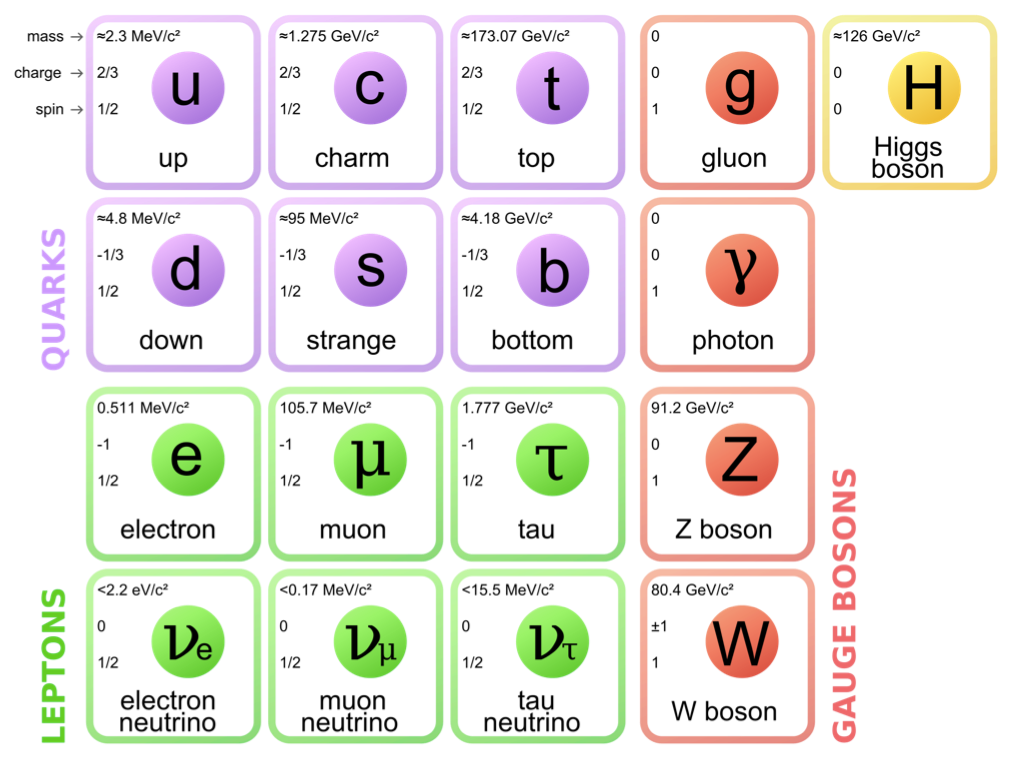
\includegraphics[width=0.8\textwidth]{Introduction/figs/SM.png}
\caption{A scheme of the fundamental particles in the SM with their properties~\cite{SM_particles}.}
\label{fig:SMparticles}
\end{figure}

Due to the asymptotic freedom of the strong interaction quarks cannot be observed alone but
are always combined with other quarks to form color singlets~\cite{Gross:1973id}. Non-fundamental particles
composed of quarks are called hadrons and are classified into two groups: mesons, where the color singlet
is achieved by the combination of a quark and an antiquark (\quark\quarkbar), and baryons
formed from three quarks (\quark\quark\quark) of different colours.
Recently, in 2014 and 2015 evidence for new states, formed by four and five quarks, was found~\cite{Aaij:2014jqa,Aaij:2015tga}.
%Recently evidence for particles composed by 4 quarks was also found~\cite{}.


\section{The electroweak interaction}
\label{sec:EMandEW}

The electromagnetic interaction is responsible for binding electrons and nuclei
together to form atoms and its mediator is the photon.
%
%,which also sets the range of the EM force to infinity, since this is proportional to the inverse of the mediator mass.
%In fact Heisenberg's Uncertainty Principle tells us that $\Delta E \Delta t > \hbar$, namely virtual particles
%of energy $\Delta E$ are allowed to exist for time intervals inferior to $\Delta t$. Thus, since particles can move
%at most at the speed of light, $c = 299792458$ ms$^{-1}$~\cite{PDG2014}, this also sets a relation between the length 
%of time and space in which a virtual photons can exist ($\Delta t > \hbar / (mc^2)$). As virtual photons can be very
%close to the mass shell, this results in a very long lifetime. The EM force has therefore an infinite range.
%
The weak interaction is responsible for the $\beta$ decay of nuclei and is mediated
by the exchange of $W^\pm$ and $Z^0$ bosons. Unlike the electromagnetic force,
that affects only charged particles, all known fermions interact through the weak interaction.
The weak interaction is also the only one that violates the parity symmetry, which states that interactions are invariant under
an inversion of spatial coordinates. This symmetry breaking arises from the fact that only left-handed fermions interact through
the weak interaction as discovered by Wu in 1957~\cite{Wu:1957my}. Similarly, the weak interaction
is the only one that also breaks the CP symmetry, which combines parity transformations and charge conjugation.
This is particularly interesting because all interactions are believed to be invariant under the CPT transformation, which combines the CP
transformation and time reversal. Hence, breaking CP the weak interaction implies that the process is also not invariant under 
time reversal transformations.

In 1968 Salam, Glashow and Weinberg unified the weak and electromagnetic forces into a single theory, where the coupling
constants of the electromagnetic, $e$, and weak, $g$, interactions are related through the weak mixing angle, $\theta_W$
by the relation $g\sin\theta_W = e$~\cite{PDG2014}. 
%
The electroweak symmetry is spontaneously broken by the Higgs
mechanism~\cite{Strocchi:1977za} and this causes the $W^\pm$ and \Z bosons to become massive (see Tab.~\ref{tab:interactions}) 
and consequently the weak force has a very short range. In fact, using Heisenberg's Principle, $\Delta E \Delta t > \hbar$, 
together with Einstein's formula $\Delta E = m c^2$, which relates mass and energy, and knowing that the maximum 
space that a particle can cover in a time $\Delta t$ is $r \sim c \Delta t$, qualitatively $r \sim \hbar / mc$. In this picture
the carriers of the weak force can travel $r \sim 2 \cdot 10^{-3}$~fm. In contrast, the photon must be massless in the theory, 
which accounts for the long range of the electromagnetic force.
%
The EW interactions are divided into Charged Currents (CC) and Neutral
Currents (NC). In the first group, quarks and leptons interact with the $W^\pm$ bosons, producing decays such as
$\mu^+(\mu^-) \rightarrow e^+ \nu_e \overline{\nu}_\mu (e^- \overline{\nu}_e \nu_\mu)$ and $n (\overline{n}) \rightarrow p e^- \overline{\nu}_e (\overline{p} e^+ \nu_e)$.
The study of these processes confirmed that only the left-handed (right-handed) component of fermions (anti-fermions)
takes part in weak processes. The CC interactions have a peculiarity: they are the only interactions in the SM that violate
flavour conservation at tree level, while any other interaction not conserving flavour has to proceed through
higher order processes. The second group of EW interactions, NC, corresponds to diagrams mediated by a photon or a \Z 
boson interacting with a fermion and its anti-fermion.



\section{Flavour and the CKM matrix}
\label{sec:flavour}

``Flavour" in particle physics refers to the quark/lepton composition of a particle. The introduction of flavour quantum numbers
was motivated in order to explain why some decays, although kinematically allowed, had never been observed. All leptons are
assigned a quantum number $L_\ell = 1$ (where $\ell = e,\mu,\tau$), which in the SM is conserved by all interactions.
This conservation is experimentally well established; for example decays like $\mu^- \rightarrow e^- \gamma $ have never
been observed.
%This is explained by the fact that the lepton number in the initial
%and final state are different and the decay would violate lepton flavour.
%
In the hadronic sector particles carry flavour numbers described as:
%
 \begin{itemize}
 \item \emph{Isospin}: $I_3 = 1/2$ for the up quark and $I_3 = -1/2$ for the down quark;
 \item \emph{Strangeness}: $S = -(n_s - \bar{n}_s)$, where $n_s$ and $\bar{n}_s$ are the numbers of strange
 and anti-strange quarks respectively;
 \item \emph{charmness, bottomness, topness}: in analogy to strangeness
 they are respectively defined as $C = -(n_c - \bar{n}_c)$, $B = -(n_b - \bar{n}_b)$, $T = -(n_t - \bar{n}_t)$.
 \end{itemize}

As mentioned previously, in the SM the only interaction violating flavour conservation is the weak interaction
when mediated by $W^\pm$ bosons.

Measuring branching fractions of weak decays like $\pi \to \mu \nu_\mu$ and $K \to \mu \nu_\mu$, corresponding
respectively to $ud\to\mu\nu_\mu$ and $us\to\mu\nu_\mu$ processes, suggested the existence of more than one
coupling constant for different quarks. Nicola Cabibbo, in order to preserve the universality
of weak interactions, suggested that the differences could arise from the fact that
the doublets participating in the weak interactions are an admixture of the mass eigenstates~\cite{PDG2014,Cabibbo:1963yz}. 
He therefore introduced the Cabibbo angle, $\theta_c$, proposing that eigenstates participating 
to the weak interaction are rotated with respect to the flavour eigenstates.
%
\begin{equation}
\left( \begin{array}{c}
d_W \\ s_W
\end{array} \right) =
\left( \begin{array}{cc}
\cos \theta_c  & \sin \theta_c\\
-\sin \theta_c & \cos \theta_c
\end{array} \right)
\left( \begin{array}{c}
d \\ s
\end{array} \right) = 
\left( \begin{array}{c}
\cos\theta_c \cdot d + \sin \theta_c \cdot s \\
\cos \theta_c \cdot s - \sin \theta_c \cdot d
\end{array} \right)
\end{equation}

In a six quark system one angle is not sufficient to describe a rotation but the mixing can be generalised
using a $3 \times 3$ unitary matrix, called the CKM matrix, from the names of Cabibbo, Kobayashi and Maskawa~\cite{Cabibbo:1963yz,Kobayashi:1973fv}.
The unitarity of the matrix is required to preserve the universality of the weak interaction. Theoretically, a $N \times N$ complex
matrix depends on $2 \cdot N^2$ real parameters. Requiring unitarity ($AA^\dagger = A(A^*)^T = I$), the number
of independent parameters left is 
\begin{equation}
(N - 1)^2 = \underbrace{\frac{1}{2}N(N-1)}_\text{Number of mixing angles} + \underbrace{\frac{1}{2}(N-1)(N-2)}_\text{Number of complex phases}.
\end{equation}  
Therefore a $3 \times 3$ matrix depends then on 4 real parameters: three real constants 
and one imaginary phase. The imaginary phase generates the \mbox{CP-violation} which was
observed in weak interactions.
Figure~\ref{fig:ch_currents_ckm} displays examples of CC processes together with the CKM elements associated with their vertices.
%
\begin{figure}[h!]
\centering 
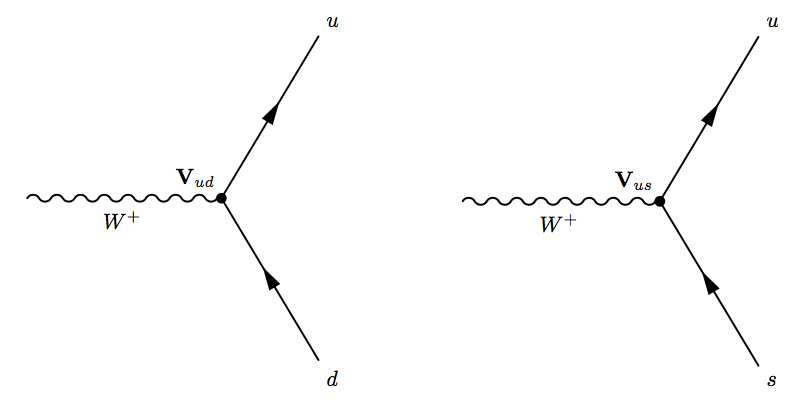
\includegraphics[width=0.6\textwidth]{Introduction/figs/ch_currents_ckm.png}
\caption{Feynman diagrams with CKM weights on weak interaction vertices as defined in Eq.~\ref{eq:CKM}.}
\label{fig:ch_currents_ckm}
\end{figure}
%
Equation~\ref{eq:CKM} reports the most recent measured values of its elements~\cite{PDG2014}
together with the widely used Wolfenstein parametrisation which highlights the hierarchical structure of the matrix.
In fact, elements on the diagonal, corresponding to transitions between quarks of the same generation,
are approximately 1 and become smaller and smaller going farther from the diagonal.
In the formula $\rho$, $A$, and $\lambda$ are the real constants and $\eta$ the imaginary phase 
and Eq.~\ref{params} shows how they are related to the three mixing angles; terms further from the diagonal 
are proportional to higher powers of $\lambda$.
%
\begin{eqnarray}
& V = \left( \begin{array}{ccc}
V_{ud} & V_{us} & V_{ub}  \\
V_{cd} & V_{cs} & V_{cb}  \\
V_{td} & V_{ts} & V_{tb}  
 \end{array} \right) = \left( \begin{array}{ccc}
0.9743 \pm 0.0002 & 0.2253 \pm 0.0007 & 0.0035^{+0.0002}_{-0.001} \\
 0.2252 \pm 0.0007 & 0.9734 \pm 0.0002 & 0.00412^{+0.0011}_{-0.0005} \\
 0.0087 \pm 0.0003 & 0.0404^{+0.0011}_{-0.0005} & 0.99915^{+0.00002}_{-0.00004} 
 \end{array} \right) \nonumber \\ 
& = \left( \begin{array}{ccc}
1 - \lambda^2/2 & \lambda  & A \lambda^3(\rho -i\eta) \\
-\lambda & 1 - \lambda^2/2 & A\lambda^2 \\
A \lambda^3(1 - \rho -i\eta) & A\lambda^2 & 1 
\end{array} \right) + O(\lambda^4)
\label{eq:CKM}
\end{eqnarray}
%
\begin{equation}
\begin{array}{rl}
\lambda & = \sin(\theta_{12}) = \sin(\theta_c) \\
A\lambda^2 & = \sin(\theta_{23}) \\
A\lambda^3(\rho - i\eta) & = \sin(\theta_{13})e^{i\delta}
\end{array}
\label{params}
\end{equation}
%
%
%Another feature to note is that, due to the unitarity of the matrix, the transformation has no effect on neutral interactions.
%
%In fact defining $q' = Vq$:
%
%\begin{equation}
%\bar{q}'q' = \bar{q}V^{*}Vq = \bar{q}q.
%\end{equation}
%
%As a result flavour-changing neutral currents are forbidden at tree level in the SM.
%

The unitarity of the CKM matrix imposes constraints to its elements of the form:
\begin{equation}
\sum_i |V_{ik}|^2 = 1 \text{ and } \sum_k V_{ik} V^{*}_{jk} = 0.
\end{equation}
These correspond to constraints on three complex numbers, which can be viewed
as the sides of triangles in the $(\rho,\eta)$ plane; these are called ``unitarity triangles".
The most commonly used unitarity triangle arises from $V_{ud}V^*_{ub} + V_{cd}V^*_{cb} + V_{td}V^*_{tb}=0$.
%\begin{equation}
%V_{ud}V^*_{ub} + V_{cd}V^*_{cb} + V_{td}V^*_{tb}=0.
%\end{equation}
Figure~\ref{fig:unitarity_triangle} shows a representation of such triangle together with
a plot summarising the most up-to-date experimental constraints to its parameters~\cite{Charles:2015gya}.
Due to these unitarity constraints flavour-changing neutral currents
are forbidden at tree level in the SM.

The precise measurement of the parameters of the CKM matrix
is a powerful stability test of the SM and sets a solid basis for new physics
searches in the flavour sector. One of the main goals of the LHCb experiment is to measure precisely
 the angle $\gamma$, which is currently the least constrained by measurements.
 %
\begin{figure}[h!]
\centering 
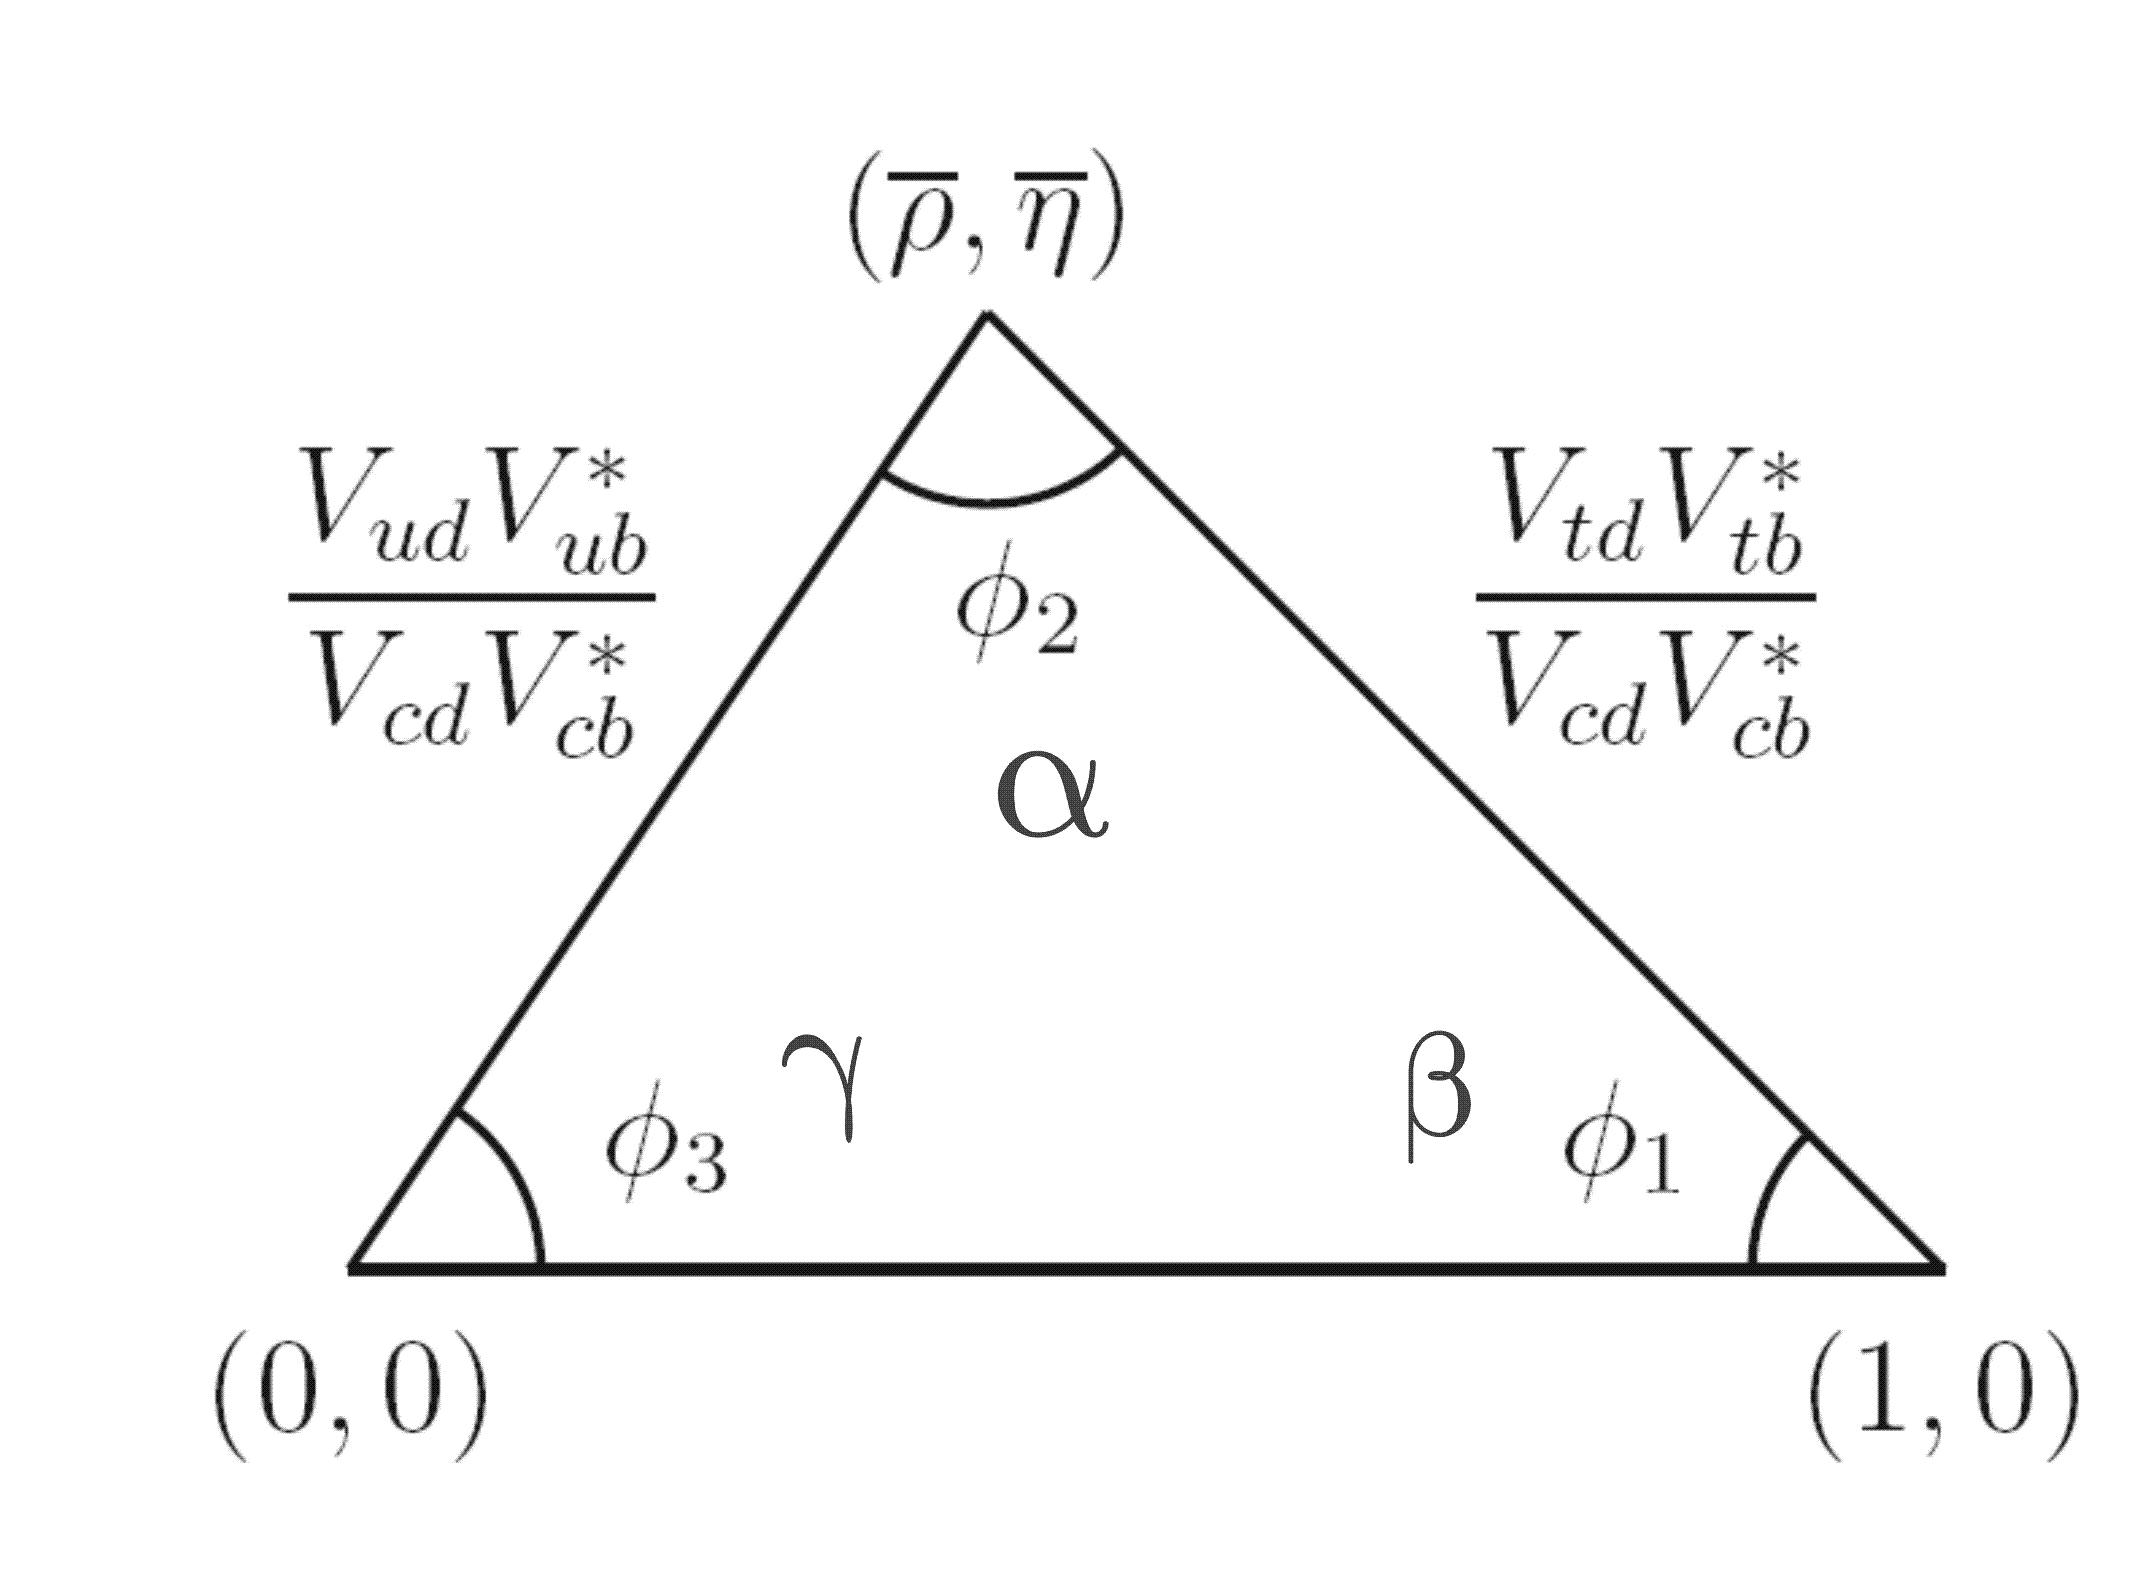
\includegraphics[width=0.5\textwidth]{Introduction/figs/Unitarity_triangle.png}
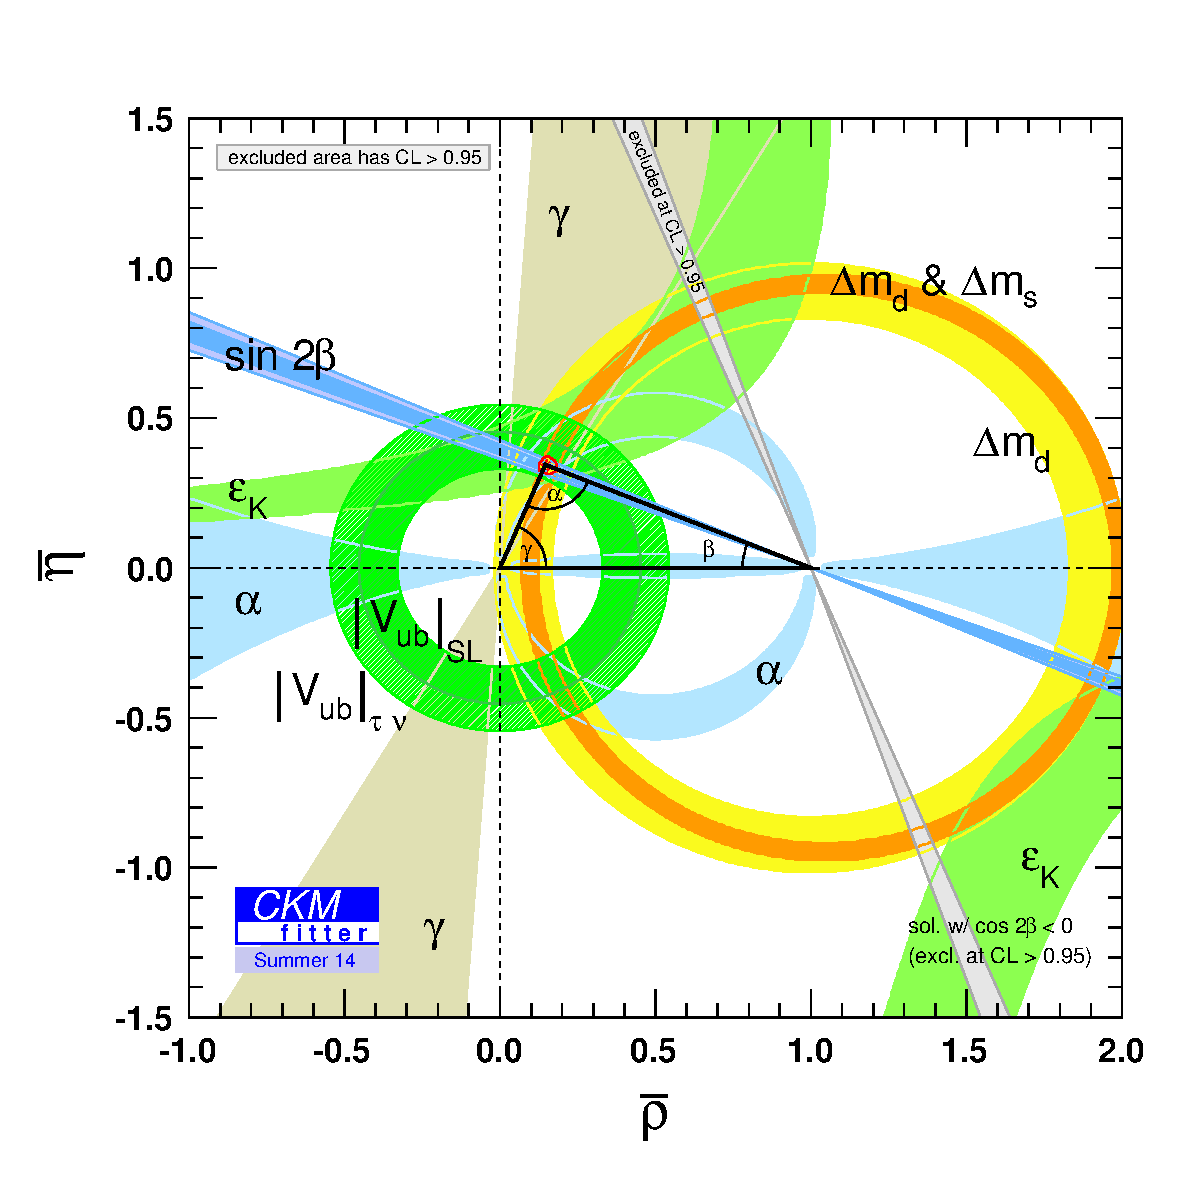
\includegraphics[width=0.7\textwidth]{Introduction/figs/Unitarity_triangle_HFAG.pdf}
\caption{(top) A representation of the unitarity triangle and its parameters.
(bottom) A summary of the most up-to-date measurements of the unitarity triangle parameters~\cite{Charles:2015gya}.}
\label{fig:unitarity_triangle}
\end{figure}
 
 
 
 
\section{The puzzles of the SM}
\label{sec:SMproblems}

Despite the experimental confirmation of many predictions of the SM, the theory has several limitations
and is unable to account for some well-established experimental facts:
%
\begin{itemize}
\item \emph{Dark matter}: experimental evidence tells us that the content of visible matter in the universe is not sufficient
to account for the observed rotation of galaxies~\cite{Zwicky:1933gu}. The most natural way to solve the problem
is the hypothesis of a form of matter that interacts with the gravitational field but not with the other SM interactions. 
%Furthermore, studies of the fluctuations of the cosmic microwave background indicate the existence of
%cold dark matter~\cite{Dunkley:2008ie}.
%formed of particles which do not interact through the SM forces and
%for which there is no SM candidate.
%
\item \emph{Matter-antimatter asymmetry}: a large asymmetry is observed between the quantity of matter 
and antimatter in the universe, $O(10^{-9})$. Assuming that both were equally created in the initial state of 
the universe, a condition such as the violation of the CP symmetry is necessary to account for the observed
imbalance. However, the magnitude of CP violation predicted by the SM, $O(10^{-20})$, is not sufficient to 
account for the observed asymmetry~\cite{Gavela:1993ts}.
%
\item \emph{Gravity}: even though the gravitational force was the first to be discovered 
this is not included in the SM. % as it can be neglected at the EW scale. 
When introducing gravity in the framework of QFT the
theory diverges. On the other hand gravity becomes irrelevant for the small masses 
of particles and can be neglected to a good approximation at the EW energy scale.
Many attempts have been made but there is not yet a consistent theoretical framework through which
 gravity can be introduced in the SM~\cite{Carlip:2001wq}. 
%
\item \emph{Neutrino oscillation}: measurements of solar and atmospheric neutrinos, as well as
neutrinos from nuclear reactors, have established that neutrinos can change flavour while propagating in space.
This is not predicted in the SM, in fact in the SM neutrinos are massless, while an oscillation requires a non-zero
 mass~\cite{Maltoni:2011zz,Cleveland:1998nv,Fukuda:1998mi,Eguchi:2002dm}.
%
\item \emph{The hierarchy problem}: the mass of a scalar (spin 0) particle, such as the Higgs boson,
suffers from quantum corrections due to the physics at high energy scales. As new physics can appear
anywhere up to the Planck scale, $\sim 10^{19}$~\gev, at which gravity cannot be neglected any more,
these corrections can be very large and it would require a high level of fine-tuning for them to cancel 
out and give such a small value as the one measured for the
Higgs Mass, $\sim 126$~\gevcc~\cite{Feng:2013pwa,Aad:2012tfa}. 
%This is considered unnatural by many physicists and pushes them
%to look for further motivations.
%
\end{itemize}
%
In conclusion, even though the SM has been very successful in describing the properties of the observed particles
and their interactions so far, because of its many puzzles, it is believed only to be part of a more general theory 
or only to be valid up to a certain energy scale. %Many theoretical models expect New Physics (NP) to enter at the TeV scale.

\subsection{The flavour problem}

%As mentioned in Sec.~\ref{sec:flavour}, flavour conservation is well experimentally established but it does not
%have a strong theoretical otivation in the Standard Model.
Flavour Changing Charged Currents (FCCC) that are mediated by the $W^\pm$ bosons are the only sources of flavour changing interaction 
in the SM and, in particular, of generation changing interactions, where a quark or a lepton of a family transforms
into one of an other family. Another class of processes is the Flavour Changing Neutral Currents (FCNCs), e.g. transitions from a
\bquark quark with a charge of -1/3 to a \squark or \dquark quark with the same charge. Examples of FCNC transitions in the quark
and lepton sector are shown in Fig.~\ref{fig:neutr_curr}.
%
\begin{figure}[h!]
\centering 
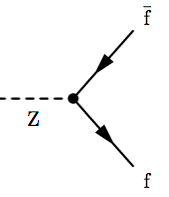
\includegraphics[width=0.25\textwidth]{Introduction/figs/Z2ffbar.png}
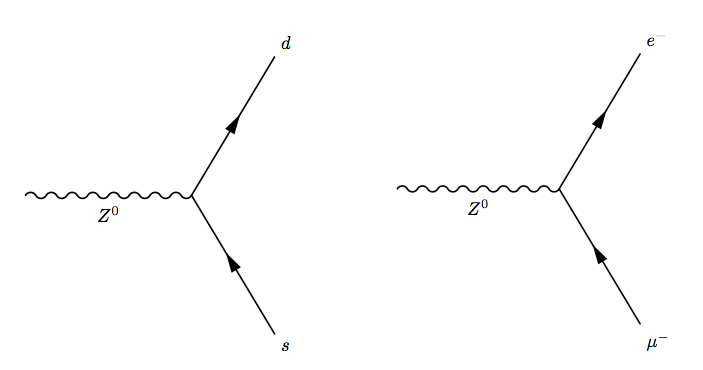
\includegraphics[width=0.6\textwidth]{Introduction/figs/neutral_current_proc.png}
\caption{Feynman diagrams of a neutral current allowed in the SM (left), where$f$ represents any fermion,
and FCNCs processes forbidden in the SM (center-right).}
\label{fig:neutr_curr}
\end{figure}
%
FCNCs are experimentally observed to be highly suppressed which derives from the unitarity of the CKM matrix,
however there is no fundamental reason why there cannot be FCNCs at tree level. In fact the CKM matrix
could be part of a larger matrix involving for example quark-lepton terms. This would introduce
new sources of FCNCs but could also allow for natural explanations of the equality of the proton and electron charges.
Furthermore, the observation of neutrino oscillation proves that flavour is not always conserved
suggesting flavour structures beyond the SM. Finally, the values of the terms of the CKM matrix and the PMNS
matrix~\cite{Pontecorvo:1967fh,Maki:1962mu}, which is the mixing-matrix equivalent to the CKM in the lepton sector,
are not explained in the SM but have to be measured experimentally. These open problems motivate searches for flavour
symmetries and deeper motivations for flavour conservation. 

\section{Beyond the Standard Model}

From the previous sections it is evident that, despite the great success of the SM, there is a need to explore theories Beyond the SM (BSM).
Among the most promising approaches there are those involving Super-Symmetry (SUSY)~\cite{Fayet:1976cr} and extra-dimensions~\cite{Randall:1999ee}. 
%
In SUSY new degrees of freedom are introduced to suppress the diverging terms of the Higgs mass. This theory
assumes that for each fermion there is a corresponding boson and, since bosons and fermions contribute with opposite
sign to the mass term, these would naturally cancel out. Supersymmetry also provides a candidate for dark
matter. In fact the lightest Super-Simmetric particle, the neutralino, which in R-parity~\cite{Ellis:1984gi} conserving variants
of the theory must be stable, is a weakly interacting potentially heavy particle.
%
The idea to introduce extra-dimensions was triggered by the fact that gravity is not relevant in particle physics but it would 
be natural if all forces had similar strength. By adding extra dimensions to the normal three spatial dimensions, one can restore 
the strength of gravity, as this could be dispersed by the wider space available.
%
In all these approaches constraints to masses and couplings must be imposed to maintain
compatibility with the SM at the electroweak scale and the existing experimental observations.

\subsection{Flavour and BSM theories}

Most BSM theories predict processes violating flavour conservation. Therefore, the observation or
non-observation of these processes can give important information about new physics.
BSM theories can be classified according to the amount of flavour violation they introduce.
The first class of models to consider is that with Minimal Flavour Violation (MFV).
These are models in which the only sources of flavour changing transitions are governed by the
CKM matrix and the CKM phase is the only source of CP violation.
This definition is driven by the fact that usually a solution of the hierarchy problem is expected
at the TeV scale, while the very small amount of flavour violation observed in measurements
seems to indicate that the SM would remain valid up to much higher energy scales.
It is therefore assumed that new physics must respect flavour symmetry principles, which also makes these
types of models naturally compatible with the SM. Examples of such models include the MSSM
with minimal flavour violation and the SM with one extra-dimension. Reviews of MFV models
are presented in Refs.~\cite{Isidori:2012ts,Buras:2003jf}.
%
%The MFV hypothesis provides a way to resolve the tension between expectation, driven by naturalness arguments,
%that NP should be at the \tev~scale and limits on FCNC processes that point to much higher scales.
%
A powerful test of MFV is provided by the study of ratios between $\bquark\to\dquark$ and $\bquark\to\squark$
transitions, because their hamiltonians share the same structure. One particularly important example is the ratio between the 
decay rates of $\Bz$ and $\Bs$ into dimuons~\cite{TomRDreview}, as this is a purely leptonic decay free from hadronic uncertainties.
In the SM such ratios are approximately equal to $|V_{td}/V_{td}| \sim 1/25$, only modified by phase space and hadronic
matrix elements, while they can take very different values in non-MFV models.

In the quest for new physics an important role is also played by simplified models
as an intermediate model building step. Instead of constructing theories valid up to the GUT scale
one can consider simplified models, where the SM is extended by the addition of new degrees of freedom
with a limited number of parameters. Such models are easier to constrain but can nevertheless point
in the right direction to build more complete theories. The choice of the new sector to add can be driven 
by the need to explain existing tensions between measurements and SM predictions or by theoretical prejudice.
%
Two models especially relevant when studying rare decays, which are the main topic of this thesis, are 
$Z'$-penguins and leptoquarks. A $Z'$-penguin is a FCNC process involving a neutral field arising from an extra 
U(1) gauge symmetry, for example U(1)$_{B-L}$, where B and L are the baryon and lepton numbers. 
As for the SM penguins, the $Z'$ field contributes in loops causing modifications of the 
effective couplings with respect to the SM. A survey of $Z'$ models can be found in Ref.~\cite{Buras:2014zga}.
%
Leptoquarks are bosonic particles that carry both quark and lepton flavour quantum numbers, which
for simplicity are assumed to be scalar.
A tree level exchange of a leptoquark induces processes such as $\bquark \to (\squark,\dquark)\ell^+\ell^-$,
and therefore can result in an enhancement of their decay rates with respect to the SM~\cite{Hiller:2014yaa}.
Leptoquarks would also provide a natural explanation for non-universal couplings to leptons.


\section{Rare decays: a tool to search for new physics}
\label{sec:RD_theory}

In the Standard Model FCNC processes are forbidden at tree level but
can occur through loop diagrams such as penguin or \W box diagrams (see Fig.~\ref{fig:penguins}).
The branching fractions of decays going through these processes are small, typically \mbox{$\sim10^{-6}$} 
or lower, and therefore they are called ``rare decays". Additional contributions to the virtual loops
are not necessarily suppressed with respect to the SM component which makes these decays
very sensitive to new physics. This approach to new physics searches is interesting as
new particles could be at high mass scales that are not accessible via direct production at colliders
but their effect could be observed in loops.
Radiative and penguin decays are particularly interesting because they are theoretically
well understood, which allows precise comparisons with measurements. Furthermore, they provide
a large quantity of observables that can be affected by new physics, not only decay rates, but also 
CP asymmetries and angular observables such as forward-backward asymmetries. The joint
analysis of different observables can help to build a consistent picture and rule out specific models.
%
\begin{figure}[h!]
\centering
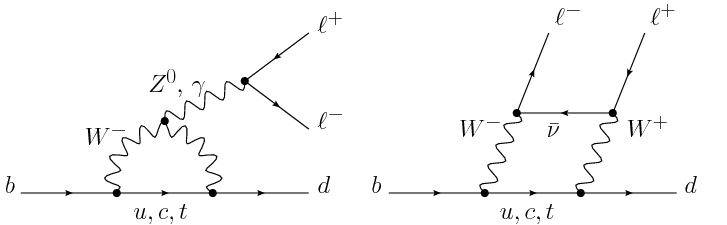
\includegraphics[width=0.9\textwidth]{Introduction/figs/penguin_general.png}
\caption{Loop Feynmann diagrams allowing $\bquark \to \dquark$ FCNC 
processes: penguin diagram (left) and \W box (right).}
\label{fig:penguins}
\end{figure}

\subsection{Theoretical framework: the effective Hamiltonian}
\label{sec:Effective_Hamiltonian}

Rare decays of \bquark hadrons are governed by an interplay between weak
and strong interactions.
%The QCD corrections that arise from hard gluon exchange bring large logarithms
%of the form $\alpha_s^n(m_b)\log^m(m_b/M)$, where $M = m_t$ or $M = m_W$.
%A suitable framework to achieve the necessary resummation of these logarithms
%in an effective low-energy theory with five quarks.
%The QCD corrections that arise from hard gluon exchange bring large contributions
%large logarithms of the form $\alpha_s^n(m_b)\log^m(m_b/M)$, where $M = m_t$ or $M = m_W$.
The large masses of the $W^\pm$ and $Z^0$ bosons and top quark compared to that of the \bquark quark allow
the construction of an effective theory that divides the problem of calculating
weak decay amplitudes into two parts: ``short-distance" and ``long-distance" effects separated
at an energy scale $\mu$. The first part, dealing with short distance physics, handles
perturbative contributions due to energy scales above the \bquark mass. The second part
typically deals with non-perturbative contributions. 
A classic example of an effective theory is the Fermi theory of weak interactions
which describes the $\beta$ decay in terms of a four-fermion interaction,
where the short distance physics is hidden into a point-like vertex as illustrated in Fig.~\ref{fig:fermi_theory}.
\begin{figure}[h!]
\centering
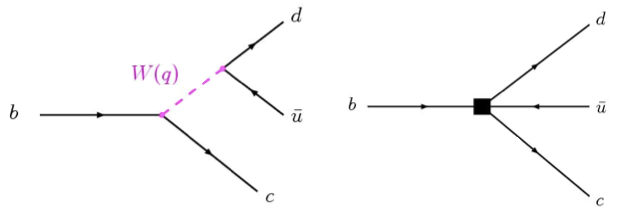
\includegraphics[width=0.7\textwidth]{Introduction/figs/fermi_theory.png}
\caption{Example of a Fermi theory in which the full theory (left) is divided into (right) a
short distance contribution, hidden in the vertex, and a long distance contribution.}
\label{fig:fermi_theory}
\end{figure}
\clearpage
The effective hamiltonian~\cite{Chetyrkin:1996vx} relevant to
$\bquark\to\squark/\dquark \gamma$ and  $\bquark\to\squark/\dquark \ell^+\ell^-$
transitions can be written as:
%
\begin{equation}
\mathcal{H}_{eff} = \frac{-4G_F}{\sqrt{2}} \left[ \lambda^t_q \sum C_i(\mu,M)\mathcal{O}_i(\mu)
+ \lambda^u_q \sum C_i(\mu,M)(\mathcal{O}_i(\mu) - \mathcal{O}_i^u(\mu)) \right],
\end{equation}
%
where $G_F$ denotes the Fermi coupling constant and the $\lambda$ constants are the CKM factors,  
$\lambda^t_q = V_{tb}V_{tq}^*$ and  $\lambda^u_q = V_{ub}V_{uq}^*$. In $\bquark\to\squark$ quark transitions, 
which are the main topic of this thesis, the doubly Cabibbo-suppressed contributions can be neglected as 
$\lambda^u_s << \lambda^t_s$. To obtain this formula the Operator Product Expansion (OPE)~\cite{Buchalla:1995vs} method
is used, which implements a summation over all contributing operators weighted by corresponding constants
called Wilson coefficients. In this Hamiltonian the long-distance contributions are described by the 
operators, $\mathcal{O}_i$, while the short-distance physics is encoded in the Wilson 
Coefficients, $C_i$. Operators and coefficients are evaluated at the renormalisation scale $\mu$.
Any particle that contributes to the decay and has a mass greater than the scale $\mu$ will affect the value 
of at least one of the Wilson coefficients, including SM particles as the top quark.

In order to describe SM processes the effective theory must be matched with the SM by requiring 
the equality between each term in effective theory and the full theoretical calculation at a matching 
scale, typically the EW scale ($\mu_W$). Then, using the scale independence of the
effective Hamiltonian, one can derive a renormalisation group equation for the Wilson Coefficients~\cite{Buras:1998raa}.
%
%
%\begin{equation}
%\mu \frac{\deriv}{\deriv \mu} C_i(\mu) = \gamma_{ij}C_j(\mu),
%\end{equation}
%
%where the matrix $\gamma$ is the anomalous dimensions matrix of the operators $\mathcal{O}_i$.
%At leading order the solution is given by~\cite{Buras:1998raa}:
%
%\begin{equation}
%C_i(\mu) = \left[ \frac{\alpha_s(\mu_W)}{\alpha_s(\mu)}\right]^{\frac{\gamma^0_{ii}}{2\beta_0}} C_i(\mu_W) = \left[ \frac{1}{1 + \beta_0\frac{\alpha_s(\mu)}{4\pi}ln\frac{\mu_W^2}{\mu^2}} \right]^{\frac{\gamma^0_{ii}}{2\beta_0}} C_i(\mu_W),
%\end{equation}
%
%where $\alpha_s$ is the strong coupling constant.
%
Taking into account only SM contributions and using $\mu_W = m_b$, the Wilson Coefficients have values:
%
\begin{equation}
\begin{array}{ccc}
C_7^{SM} = -0.3, & C_9^{SM} = 4.2, & C_{10}^{SM} = -4.2
\end{array}
\end{equation}
%
and new physics contributions appear in the Wilson Coefficients in the form of additive factors:
\begin{equation}
 C_i = C_i^{NP} + C_i^{SM}.
\end{equation}

The amplitudes of exclusive hadronic decays can be calculated as the expectation 
values of the effective Hamiltonian. Given an initial state $I$ and a final state $F$
\mbox{(e.g. $I = \Bz$ and $F=\Kstarz\mumu$)} the decay amplitude can be calculated as
%
\begin{equation}
\begin{array}{rl}
A(I\to F) &= \langle I | \mathcal{H}_{eff} | F \rangle = \\
&= \frac{G_F}{\sqrt{2}} \sum V_{CKM}^i \underbrace{C_i(\mu)}_{\shortstack{Perturbative \\ Includes new physics}} \cdot  \underbrace{\langle I | \mathcal{O}_i(\mu) | F \rangle}_{\shortstack{Non-preturbative \\ Known physics}},
\end{array}
\end{equation}
where $\langle I | \mathcal{O}_i(\mu) | F \rangle$ are the hadronic matrix elements also called  ``form factors".
These can be evaluated using non perturbative methods such as lattice calculations.
However, due to the limitations of these methods, they represent the dominant source 
of uncertainty in theoretical calculations.

\subsection{Operators}
\label{sec:operators}

Separating the left- and right-handed components the effective Hamiltonian is
%for $\bquark\to\squark\ell^+\ell^-$ transitions is
%
\begin{equation}
\mathcal{H}_{eff} = \frac{4G_F}{\sqrt{2}} V_{tb}V^*_{ts} \frac{\alpha_e}{4\pi} \sum_{i=1}^{10} \left[ C_i \mathcal{O}_i  +  C'_i \mathcal{O}'_i \right].
\end{equation}
%
%where the $V_{ub}$ and $V_{bs}$ are the factors of the CKM matrix.
A complete basis is given by a set of 10 operators, where $\mathcal{O}_{1,2}$ are the tree level W operators;
$\mathcal{O}_{3-6,8}$ are penguin diagrams mediated by gluons; and $\mathcal{O}_{7,9,10}$, which are the operators
that are relevant for radiative and leptonic penguin processes are defined as~\cite{TomRDreview}:
%S is Higgs scalar penguins and P pseudo-scalar penguin
%
\begin{equation}
\begin{array}{ll}
 \mathcal{O}_7 = \frac{m_b}{e} (\bar{s} \sigma^{\mu\nu}P_Rb)F_{\mu\nu},  		& \mathcal{O}_7' = \frac{m_b}{e} (\bar{s} \sigma^{\mu\nu}P_Lb)F_{\mu\nu}, \\
%\mathcal{O}_8 = g_s\frac{m_b}{e} (\bar{s} \sigma^{\mu\nu}P_RT^ab)G^a_{\mu\nu}  	& \mathcal{O}_8' = g_s\frac{m_b}{e} (\bar{s} \sigma^{\mu\nu}P_LT^ab)G^a_{\mu\nu} \\
\mathcal{O}_9 = (\bar{s} \gamma_{\mu}P_Lb)(\bar{\ell}\gamma^\mu\ell), 			& \mathcal{O}_9' = (\bar{s} \gamma_{\mu}P_Rb)(\bar{\ell}\gamma^\mu\ell), \\
\mathcal{O}_{10} = (\bar{s} \gamma_{\mu}P_Lb)(\bar{\ell}\gamma^\mu\gamma_5\ell), 	& \mathcal{O}_{10}' = (\bar{s} \gamma_{\mu}P_Rb)(\bar{\ell}\gamma^\mu\gamma_5\ell),
\end{array}
\end{equation}
%
where $P_{L/R} = (1 \mp \gamma_5)/2$ denote the left- and right-handed chiral projections 
%$T^a$ are the QCD generators 
and $F_{\mu\nu}$ is the electromagnetic field tensor.
%
The $\mathcal{O}'$ operators correspond to right-handed coupling obtained by swapping
$P_R$ and $P_L$ in the equations. In the SM, as well as in MFV models where the
flavour violation is entirely ruled by the CKM matrix, the $C'$ Wilson Coefficients 
are suppressed by the strange coupling, $C'_i \sim (m_s / m_b) C_i$.
%
The operator $\mathcal{O}_7$ relates to penguin diagrams that are mediated via a photon.
%and the $\mathcal{O}_8$ by a gluon. The $\mathcal{O}_7$ operator is 
It represents the dominant contribution to the radiative 
$\bquark\to\squark\gamma$ transition and contributes to $\bquark\to\squark\ell^+\ell^-$ processes when
the virtual photon decays into a dilepton pair. The semileptonic $\mathcal{O}_9$ and $ \mathcal{O}_{10}$ 
correspond to penguin diagrams mediated by a $Z^0$ boson and $W$ mediated box diagrams. 
These are the dominant contributions in semileptonic $\bquark\to\squark\ell^+\ell^-$ decays.
The vertices corresponding to the radiative and semileptonic operators are illustrated in Fig.~\ref{fig:vtx_operators}
%
\begin{figure}[h!]
\centering
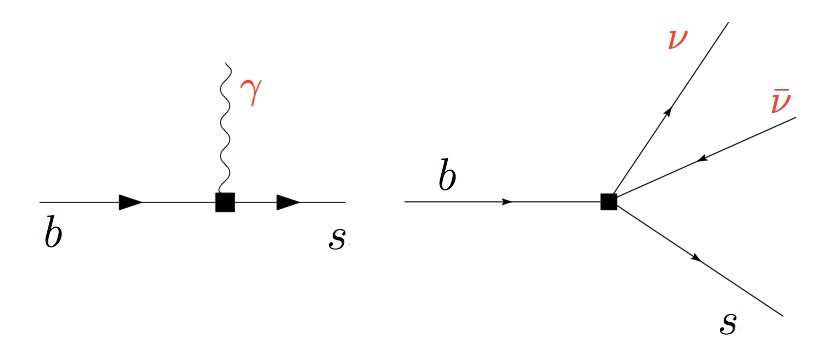
\includegraphics[width=0.6\textwidth]{Introduction/figs/vtx_operators.png}
\caption{Interaction vertices corresponding to the radiative (left) and semileptonic (right) operators.}
\label{fig:vtx_operators}
\end{figure}

It is also common to express the semileptonic operators in a basis with left and right projected leptons
%
\begin{equation}
\begin{array}{ll}
\mathcal{O}_{LL} = ( \mathcal{O}_{9} - \mathcal{O}_{10})/2 & \mathcal{O}_{LR} = ( \mathcal{O}_{9} + \mathcal{O}_{10})/2 \\
\mathcal{O}_{RR} = ( \mathcal{O}'_{9} - \mathcal{O}'_{10})/2 & \mathcal{O}'_{RL} = ( \mathcal{O}'_{9} + \mathcal{O}'_{10})/2 \\
\end{array}
\end{equation}
%
where the Wilson Coefficients are redefined as
\begin{equation}
\begin{array}{ll}
C_{LL} = C_{9} - C_{10}, & C_{LR} =  C_{9} + C_{10}, \\
C_{RR} = C'_{9} - C'_{10}, &C'_{RL} =  C'_{9} +C_{10}. \\
\end{array}
\end{equation}
%
This basis is particularly useful in frameworks where BSM physics at a high mass scale
respects the SU(2)$_W$ part of the SM gauge symmetry group.
%For instance, instead of fitting the two parameters $C_9$
%and $C_{10}$, the LL-hypothesis gives the constraint $C_9 + C_{10} = 0$.
%since C9 +C10 = 0 in the standard model there is no sensitivity to CLR and 
%CRR from interference with the standard model in semileptonic decays.
%
Finally, in the picture presented in this section all operators were considered as universal
with respect of the flavour of the involved leptons. However, BSM models often contain sources of
lepton universality violation leading to a split of the same operators depending on the lepton considered:
$C_i \to C_i^e$, $C_i^\mu$, $C_i^\tau$ and $\mathcal{O}_i \to \mathcal{O}_i^e$, $\mathcal{O}_i^\mu$, $\mathcal{O}_i^\tau$. 

\subsection{Phenomenology of $\bquark\to\squark\ell^+\ell^-$ decays}
\label{sec:theo_qsq}

Semileptonic \bquark hadron decays are characterised by two kinematic regimes which
are treated theoretically in different ways; Table~\ref{tab:q2scheme} shows a scheme of the \qsq spectrum.
%
The ``high $q^2$" is the region of low hadron recoil, $\qsq > 15$~\gevgevcccc, and is characterised by 
the energy of the hadron being less than the energy scale of QCD interactions within the meson, 
\mbox{$\Lambda_{QCD} \sim 1$~\gev}. In this region theoretical calculations of $B$ meson decays can be simplified 
by working in the heavy quark limit, $m_b\to\infty$. In this limit a Heavy Quark Effective 
Theory (HQET)~\cite{DellaMorte:2015yda} can be constructed in which the heavy quark interacts 
only via `soft' hadronic processes and an OPE in $1/m_b$ is valid.
%?QCD/mb then shows that the perturbatively calculable parton-level process is the leading 
%contribution to the B0 ?K?0?+?? decay, and the hadronic effects are relatively small. 
%. A heavy-quark expansion in terms of The QCD Factori- sation (QCDF) technique separates the parton-level and %hadronic contributions at the energy scale ??mb, accounting for the ?soft? non-perturbative processes using hadronic %form factors [25].
%
%
%\begin{table}[b]
%\caption{A scheme of the \qsq spectrum.}
%\begin{tabular}{llcrr}
%{\footnotesize $\qsq = 0$ }   &  {\footnotesize  $E_{\Kstarz}  >> \Lambda_{QCD}$	}&  {\footnotesize $\qsq \sim m_{\jpsi,\psitwos}^2$ } & {\footnotesize $E_{\Kstarz}  \sim \Lambda_{QCD}$ } & {\footnotesize $\qsq = (m_B - m_\Kstarz)^2$ } \\
%\hline
%{\footnotesize max. recoil } & {\footnotesize large recoil (SCET) } & {\footnotesize $\cquark\cquarkbar$ resonances } & {\footnotesize low recoil (HQET) } & {\footnotesize zero recoil} \\
%\end{tabular}
%\label{tab:q2scheme}
%\end{table}
\begin{table}[b]
\caption{A scheme of the \qsq spectrum.}
\centering
\begin{tabular}{c|c|c|c}
 \qsq							& $E_{\Kstarz}$	   	&  	Regime 			& 	Valid theory \\ \hline
 $\sim 0$ \gevgevcccc			& $\sim m_B$			&   Max. recoil			&	\multirow{ 2}{*}{SCET}\\ 
 $< 6$	\gevgevcccc			& $>> \Lambda_{QCD}$	&	Large recoil		&		   		\\ \hline
 $\qsq \sim m_{\jpsi,\psitwos}^2$ 	& $\sim 3$ \gev			& 	$\cquark\cquarkbar$ resonances	&  -- 		\\ \hline
 $\qsq > 15$ \gevgevcccc 			& $E_{\Kstarz}  \sim \Lambda_{QCD}$ 			&	Low recoil	&	\multirow{ 2}{*}{HQET}\\
 $\qsq = (m_B - m_\Kstarz)^2$ 		& $E_{\Kstarz} \sim 0$  	&	Zero recoil		&			\\
\end{tabular}
\label{tab:q2scheme}
\end{table}
%
The \mbox{``low $q^2$"} region is where the light spectator quark is energetic and cannot be neglected.
Furthermore, the light quark interacts not only via `soft' hadronic processes, as in HQET, but also via the 
so-called `collinear' hadronic processes.
The boundary of this region can be set at $\sim 7$~\gevgevcccc~ which corresponds to the threshold for 
$\cquark\cquarkbar$ production, $(2m_c)^2$. 
In this region the hadronic interactions are handled by expanding in terms 
of the energy of the emitted energetic hadron, $1/E_h$, forming the so-called Soft-Collinear 
Effective Theory (SCET)~\cite{Bauer:2000yr}.
%
\begin{figure}[h!]
\centering
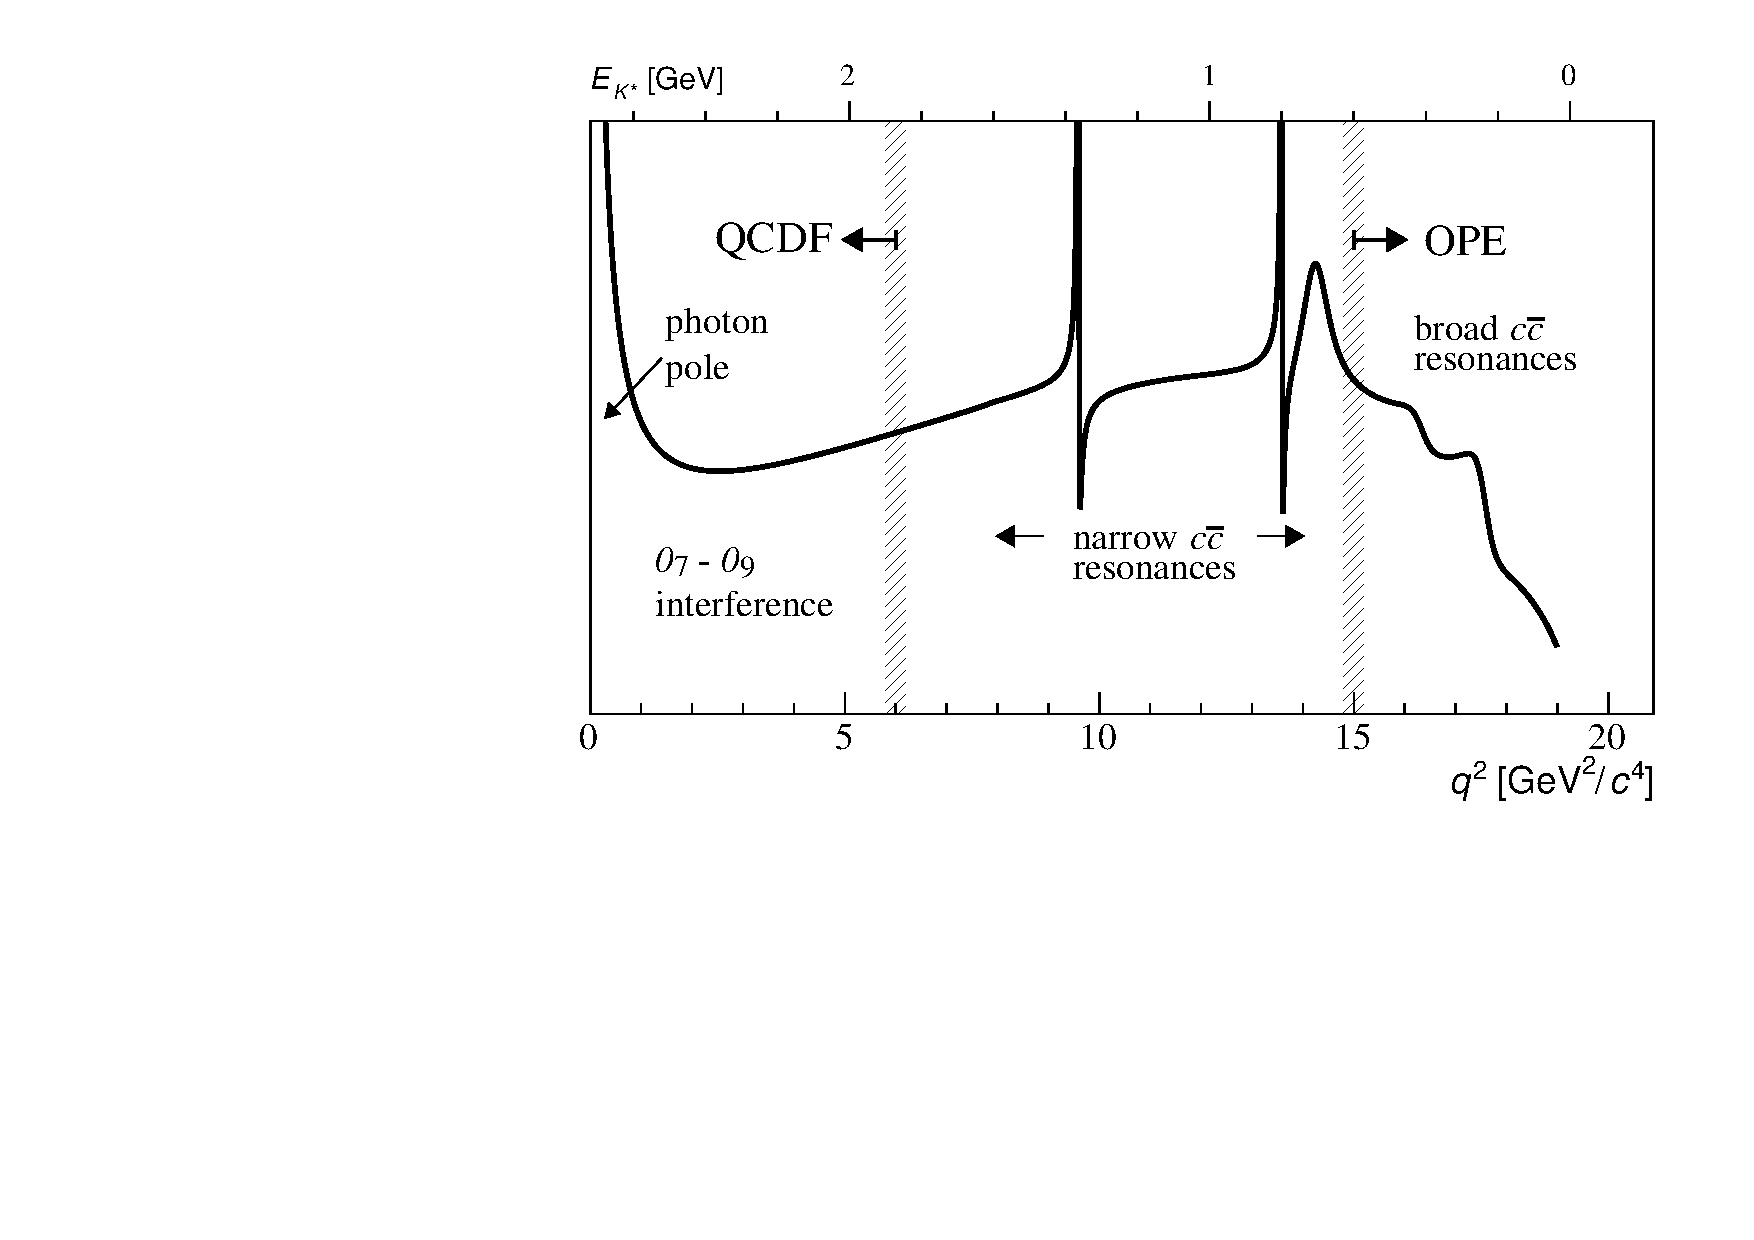
\includegraphics[width=0.8\textwidth]{Introduction/figs/q2spectrum.pdf}
\caption{A typical \qsq spectrum of $\bquark\to\squark\ll$ processes characterised by the photon pole
at  low \qsq, charmonium resonances at central \qsq and broad resonances at high \qsq~\cite{TomRDreview}.}
\label{fig:q2spectrum}
\end{figure}
%
In both regions decay rates can be predicted using the different methods and
the biggest uncertainties come from the limited knowledge of hadronic transition matrix elements.
The intermediate region is characterised by the presence of charmonium resonances, produced though tree 
level $b\to\cbar c s$ transitions and no precise theoretical calculation is available~\cite{Khodjamirian:2010vf}.

As can be seen in Fig.~\ref{fig:q2spectrum} the very low \qsq region is characterised by a peak due
to the virtual photon contribution, associated with $C_7$. In the region $1-6$~\gevgevcccc the 
interference between $C_7$ and $C_9$ becomes large, yielding sensitivity to new physics in $C_9$.
The $7-15$~\gevgevcccc interval is dominated by the charmonium resonances, \jpsi and \psitwos. 
Although these decays can be experimentally vetoed in
principle charmonia affect the entire \qsq space. Finally, at high \qsq broad charmonium resonances 
can contribute, like those observed by LHCb in $\decay{B^+}{K^+\mumu}$ decays~\cite{LHCB-PAPER-2013-039}.

\subsection{Observables in $\bquark\to\squark\ell^+\ell^-$ decays}
\label{sec:observables}

Rare decays and especially semileptonic $\bquark\to\squark\ell^+\ell^-$ processes offer a number
of observables which can be used to study BSM models.
The most direct effects appear in decay rates that can be enhanced by new physics but the precision on
these measurements is often limited by uncertainties on the non-perturbative part of the calculations.
Therefore, it is important to also look for different observables.
One important class of observables are angular quantities that can often carry complementary 
information with respect to branching ratio measurements. The most basic of these
observable are forward-backward asymmetries that characterise the angular distribution of final particles. 
For the $\Bz\to\Kstar\mumu$ decay combinations of observables have been proposed
that are independent of form factor uncertainties at leading order order~\cite{TomRDreview}.

Another way to build safe observables is to construct ratios between similar
decays, in which uncertainties due to the hadronisation process cancel out.
These observables include the $R_H$ ratios, between \Bz decays into electrons and muons,
that are described in detail in Ch.~\ref{sec:RKst_theory}.
It is also interesting to compare decays which proceed via the same fundamental process but
where the spectator quark has a different flavour. This is the case of $\Bu\to K^+\mumu$ and $\Bz\to\KS\mumu$
decays, which are both $\bquark\to\squark$ transitions where the spectator quark is an \uquark quark
in the first case and a \dquark quark in the second. The normalised difference of the branching fractions
of these decays is called isospin asymmetry.


\section{Experimental status}
\label{sec:exp_status}

To set the background for the analyses described in this thesis, this section reports a 
brief review of recent results of new physics searches involving rare decays or lepton flavour violation.
Among these, results recently obtained by the \lhcb experiment show a series of anomalies
with respect to the SM that have the potential to yield to BSM scenarios.


\subsection{Dimuon decays of \bquark hadrons}

Decays of $B$ mesons into a pair of muons are two-body decays where the two muons are back to
back in the hadron rest frame. The simple signatures of these decays makes them easy to study
and the fact that they are unaffected by hadronic physics in the final state makes predictions very
clean and precise. Therefore these are essential tests of the SM.
The $\decay{\Bz}{\mumu}$ and $\decay{\Bs}{\mumu}$ decays are FCNCs that can only happen 
via loops and furthermore they are CKM-suppressed, which makes them particularly rare.
In addition to that the decay of a pseudo-scalar $B$ meson into two muons has a significant helicity
suppression. The latest SM predictions for these decay rates are~\cite{Bobeth:2013uxa}:
%
\begin{align}
\mathcal{B}(\decay{\Bs}{\mumu}) &= (3.65 \pm 0.23) \times 10^{-9} \text{ and } \\
\mathcal{B}(\decay{\Bz}{\mumu}) &= (1.06 \pm 0.09) \times 10^{-10}.
\end{align}
%
The uncertainties on these values are dominated by the knowledge of the decay constants and 
CKM-elements. BSM models can produce significant enhancement to these decay rates
and the measurement of their ratio is a stringent test of the MFV hypothesis.
A combination of the \lhcb and \cms results measured the values~\cite{CMS:2014xfa}:
%
\begin{align}
\mathcal{B}(\decay{\Bs}{\mumu}) &= (2.8^{+0.7}_{-0.6}) \times 10^{-9} \text{ and } \\
\mathcal{B}(\decay{\Bz}{\mumu}) &= (3.9^{+1.6}_{-1.4}) \times 10^{-10}.
\end{align}
%
%
\begin{figure}[b!]
\centering
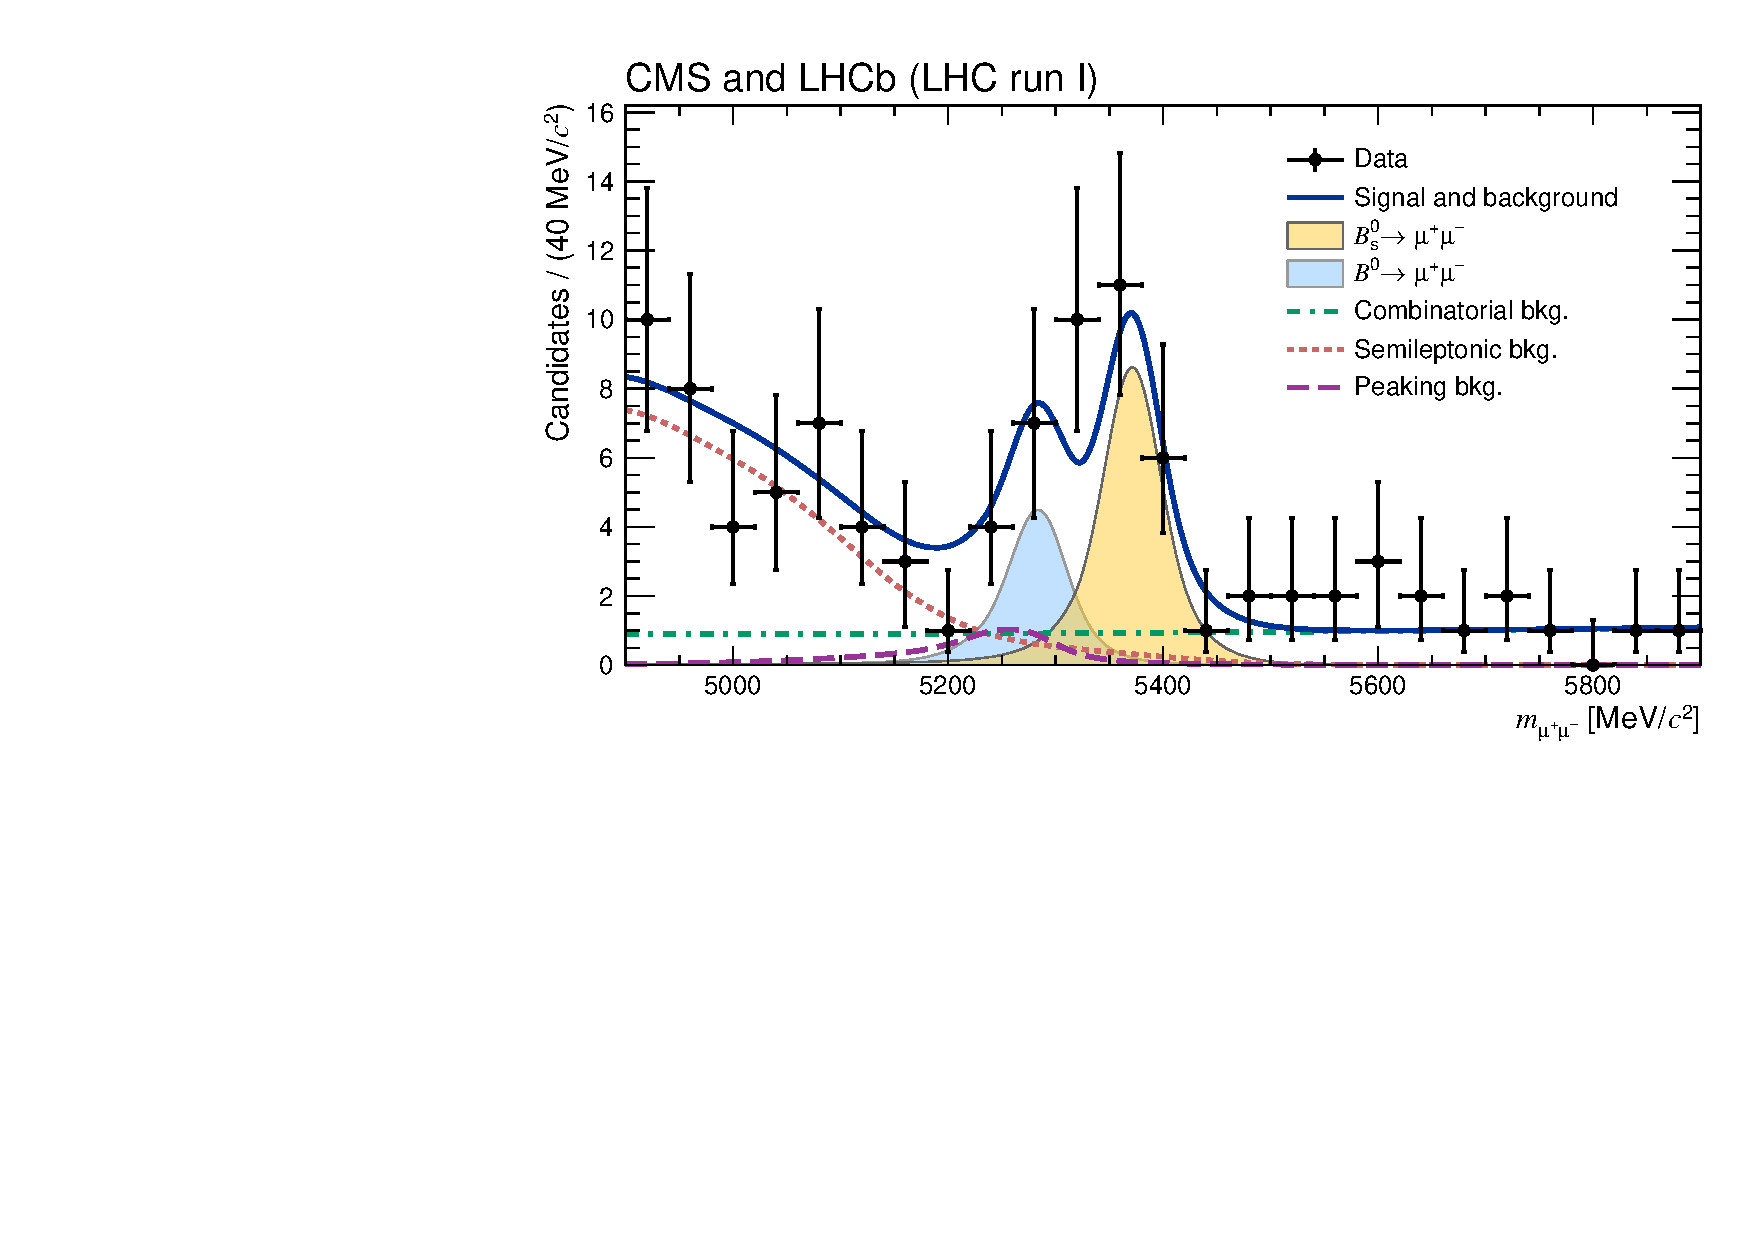
\includegraphics[width=0.6\textwidth]{Introduction/figs/CMSLHCb_EDfig2.pdf}
\caption{Dimuon invariant mass of $B$ candidates showing peaks corresponding 
$\Bs\to\mumu$ and $\Bz\to\mumu$ decays~\cite{CMS:2014xfa}.}
\label{fig:bsmumu}
\end{figure}
%
Neither decay had been previously observed, while now the $\Bs$ decay is observed
with a significance of $6\sigma$ and evidence for the $\Bz$ decay is found
at $3\sigma$ significance level. The measured branching fractions are compatible 
with SM predictions within $2\sigma$ and put strong constraints on the available 
parameter-space for BSM theories. Figure~\ref{fig:bsmumu} shows the fit the dimuon 
invariant mass of $B$ meson candidates where the peaks of the two decays are visible.

\subsection{Semileptonic $\bquark\to\squark\ell^+\ell^-$ decays of \bquark hadrons}
\label{sec:exp_btosll}

At the LHC it is possible to collect large data samples of semileptonic 
decays, especially those with muons in the final state.
Many branching fractions of semileptonic $B$ meson decays were recently measured at
the \lhcb experiment, including $\decay{B}{K\mumu}$, $\decay{B}{\Kstarz\mumu}$
and $\decay{\Bs}{\phi\mumu}$~\cite{LHCB-PAPER-2014-006,LHCB-PAPER-2013-017,LHCB-PAPER-2013-019}. 
Baryon decays were also studied at \lhcb: including 
the rare $\decay{\Lambda_b}{\Lz\mumu}$ decay~\cite{Aaij:2015xza}, whose analysis is described in this thesis.
In contrast to purely leptonic decays, SM predictions for semileptonic decays are affected by the
knowledge of hadronic form factors, which results in relatively large uncertainties,
$\mathcal{O}(30\%)$. As a result measurements are now typically more precise than predictions.

Among the measurements of angular observables that can be affected by 
new physics, particular interest was raised by the measurement of a set of observables in
$\decay{\Bz}{\Kstarz\mumu}$ decays, free from form factors uncertainties at leading order~\cite{LHCB-PAPER-2013-037}.
Most of the measurements are found to be in agreement with SM predictions
with the exception of the $P'_{5}$ observable, shown in Fig.~\ref{fig:P5prime}, which presents
a local $3.7\sigma$ deviation confirmed by a recent analysis with higher statistics~\cite{Aaij:2015oid}.
 Attempts to build a consistent picture point to a new physics contribution
to the Wilson Coefficient $C_9$~\cite{Descotes-Genon:2013wba}.
An angular analysis of $\Bu\to K^+\mumu$ decays was also performed, where observables
are found to be compatible with SM predictions~\cite{LHCB-PAPER-2014-007}.
%
\begin{figure}[h!]
\centering
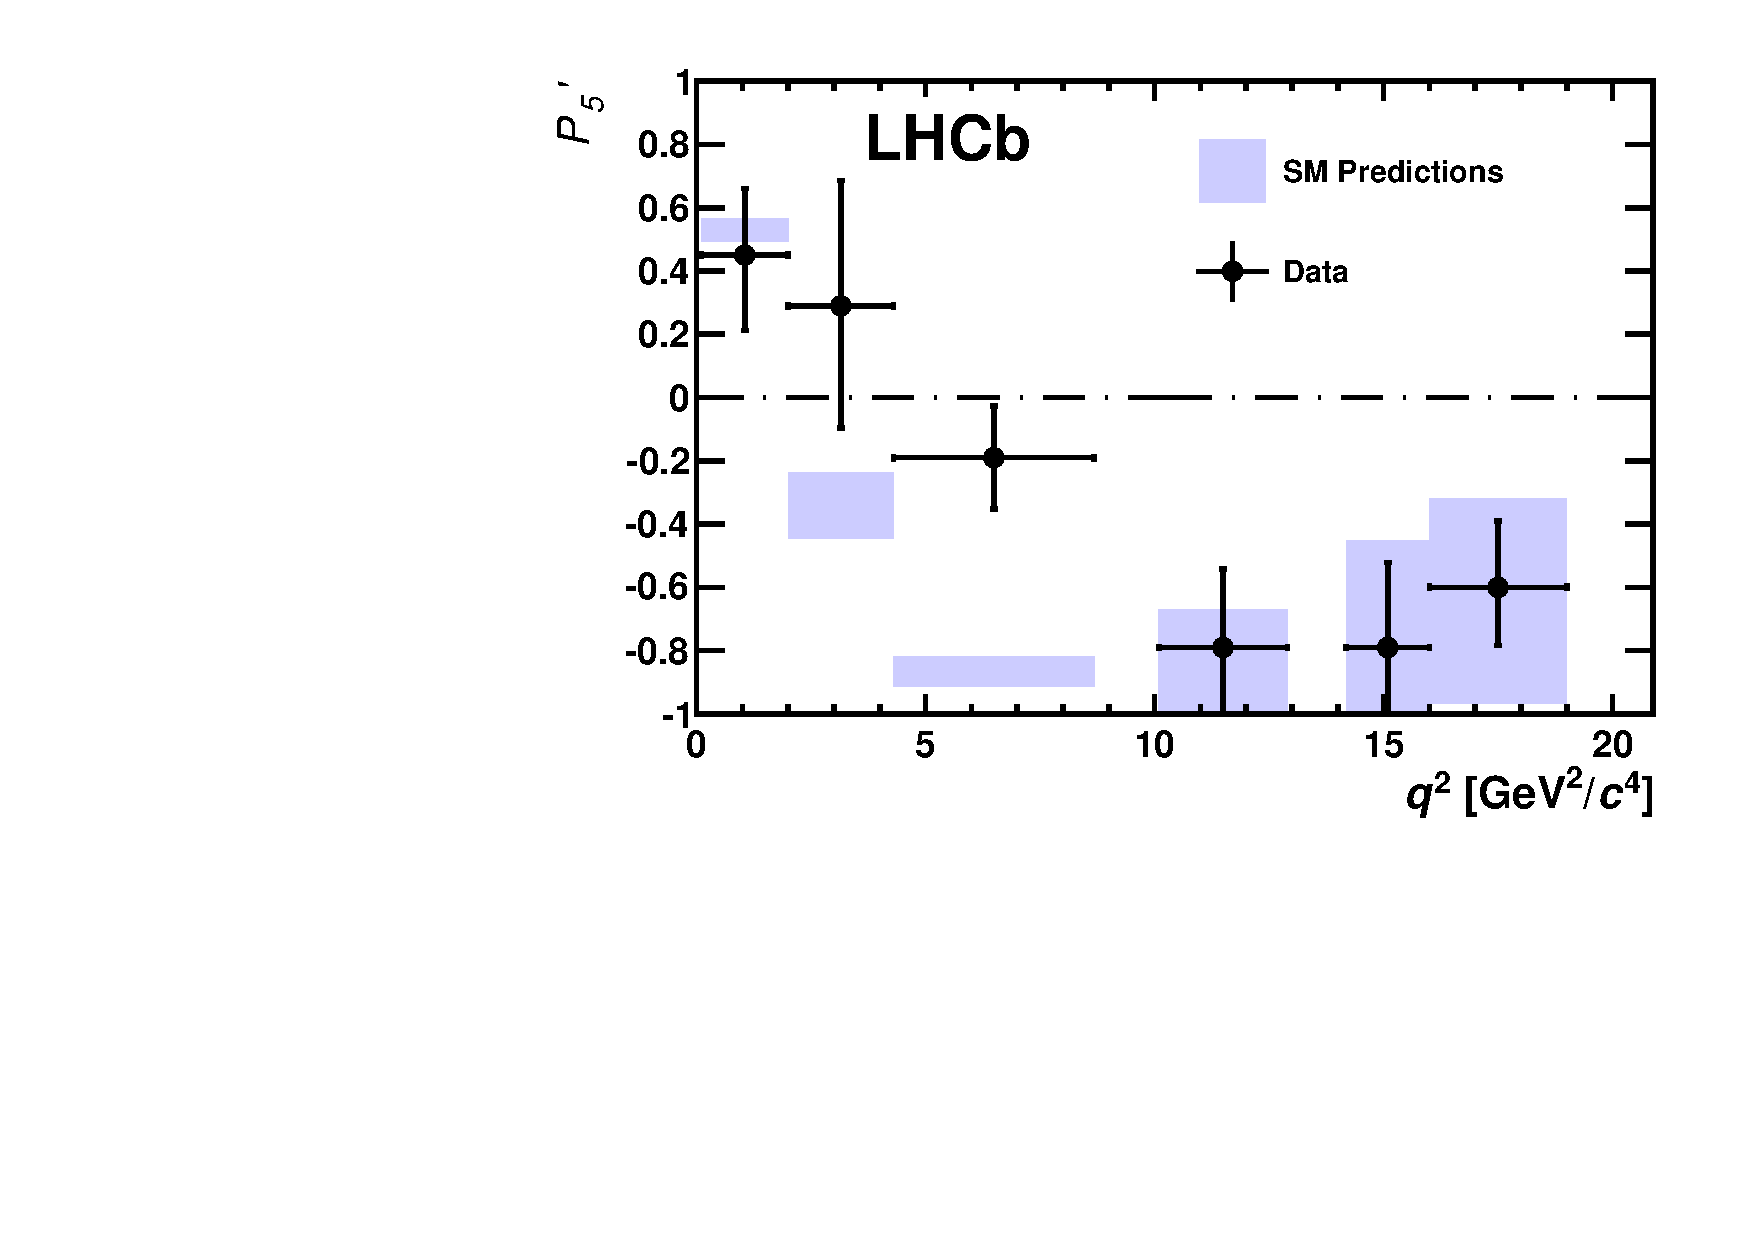
\includegraphics[width=0.6\textwidth]{Introduction/figs/P5prime.pdf}
\caption{Measurement of the $P'_{5}$ observable as a function of \qsq, showing a tension with
SM predictions in the 2--6 \gevgevcccc region~\cite{LHCB-PAPER-2013-037}.}
\label{fig:P5prime}
\end{figure}
%
Other observables for which the sensitivity to form factors effects is reduced are the CP asymmetry between
$B$ and $\bar{B}$ decays, $\mathcal{A}_{CP}$, and the isospin asymmetry between \Bz and \Bu decays, $\mathcal{A}_{CP}$.
Due to the small size of the corresponding CKM elements, CP asymmetries of $\Bz\to K^{(*)}\mumu$
decays are tiny in the SM, $O(10^{-3})$. In BSM models new sources of CP violation can arise and therefore
$\mathcal{A}_{CP}$ measurements are a powerful test of the SM. 
The isospin asymmetry is not zero in the SM due to isospin breaking effects in the form factors.
This is expected to be $\sim1$\% at low \qsq and increase to $\sim10$\% as \qsq tends to zero.
The LHCb experiment, using the full dataset collected in Run I, corresponding to an integrated luminosity of
3~\invfb and $\sim 10^9$ $B$ decays, measured both of these asymmetries to be consistent with
zero~\cite{LHCB-PAPER-2014-006,Aaij:2014bsa}, as reported in Tab.~\ref{tab:AcpAI}. 
%
\begin{table}
\begin{small}
\begin{tabular}{c|cc|cc}
\multirow{2}{*}{}	& \multicolumn{2}{c|}{$\Bz\to K^+\mumu$}			&\multicolumn{2}{c}{$\Bz\to \Kstarz\mumu$}	\\ \cline{2-5}
							& 1.1--6 	[\gevgevcccc]	& 15.0--22.0 [\gevgevcccc] & 	1.1--6 [\gevgevcccc]	& 15.0--19.0 [\gevgevcccc]			\\ \hline
$\mathcal{A}_{CP}$  & $0.004 \pm 0.028$	 				& $-0.005 \pm 0.030$		&	$0.094 \pm 0.047$	& $-0.074 \pm 0.044$ 	\\
$\mathcal{A}_{I}$	& $-0.10^{+0.08}_{-0.09} \pm 0.02$	& $-0.09 \pm 0.08 \pm 0.02$	&	$0.00^{+0.12}_{-0.10} \pm 0.02$  &	$0.06^{+0.10}_{-0.09} \pm 0.02$ \\
\end{tabular}
\end{small}
\caption{Measurement of CP and isospin asymmetry in $\Bz\to \Kstarz\mumu$ decays from the LHCb experiment~\cite{TomRDreview}.  }
\label{tab:AcpAI}
\end{table}
%
Recently, progress was made measuring also electron channels.
The branching fraction of the $\Bz\to\Kstarz\ee$ decay was measured to be $(3.1\pm1.3)\times10^{-7}$ in the dilepton mass interval 30--1000~\mevcc~\cite{LHCB-PAPER-2013-005}. Furthermore, for the first time
angular observables were measured for this decay and found to be consistent with SM predictions~\cite{Aaij:1981106}.

Given the wide set of available measurements, theorists have implemented global fits including results from rare decays analyses,
 as well as inputs from \Bs mixing and Higgs measurements, in order to understand if the existing anomalies could be caused by a common factor.
The results of such global fits agree that there is a tension with respect to the SM at the level of 1--4.2 standard deviations,
depending on the set of assumptions made. In particular they favour a shift $C^{NP} \sim -1$ to the $C_9$ Wilson
Coefficient, related with the penguin diagram mediated by a $Z^0$ boson~\cite{Altmannshofer:2014rta,Descotes-Genon:2013wba,Hurth:2016fbr}. 

\subsection{Lepton Flavour Violation searches}

Several Lepton Flavour Violation (LFV) searches are linked to rare decays as they involve small branching
ratios in the SM that can be enhanced by BSM physics. %They are therefore a natural place to look for new physics.
Lepton flavour conservation is experimentally well-established measuring the branching ratios of
decays of muons into electrons and no neutrinos, but has no strong theoretical
explanation in the context of the SM. In fact it is already observed that flavour
is not conserved in neutrino oscillations. 
%This section reports a short review of LFV searches. 
%
The best-studied decays violating lepton flavour 
are rare muon decays including $\mu^+\to e^+\gamma$ and $\mu^+\to e^+e^-e^+$.
Since muons can be abundantly produced and the final states are simple,
these decays provide the best constraints to LFV. The present best upper limits are $1.2 \times 10^{-11}$
for the radiative decay and $1.0 \times 10^{-12}$ for \mbox{$\mu^+\to e^+e^-e^+$} obtained
respectively by the MEGA~\cite{Ahmed:2001eh} and SINDRUM~\cite{Bellgardt:1987du} experiments.
Several LFV searches in the $B$ sector have recently been performed at the LHCb experiment 
including decays such as $\Bz\to e\mu$~\cite{LHCB-PAPER-2013-030} and $\tau$ decays such
as $\tau\to\mumu\mu$~\cite{LHCB-PAPER-2013-014}. None of these searches has found evidence 
of new physics so far and therefore they set limits, constraining the parameter space available for BSM models.
Figure~\ref{fig:LFV_decay} shows a summary of the best limits set at different times
on LFV searches~\cite{Marciano:2008zz}.


\begin{figure}[h!]
\centering 
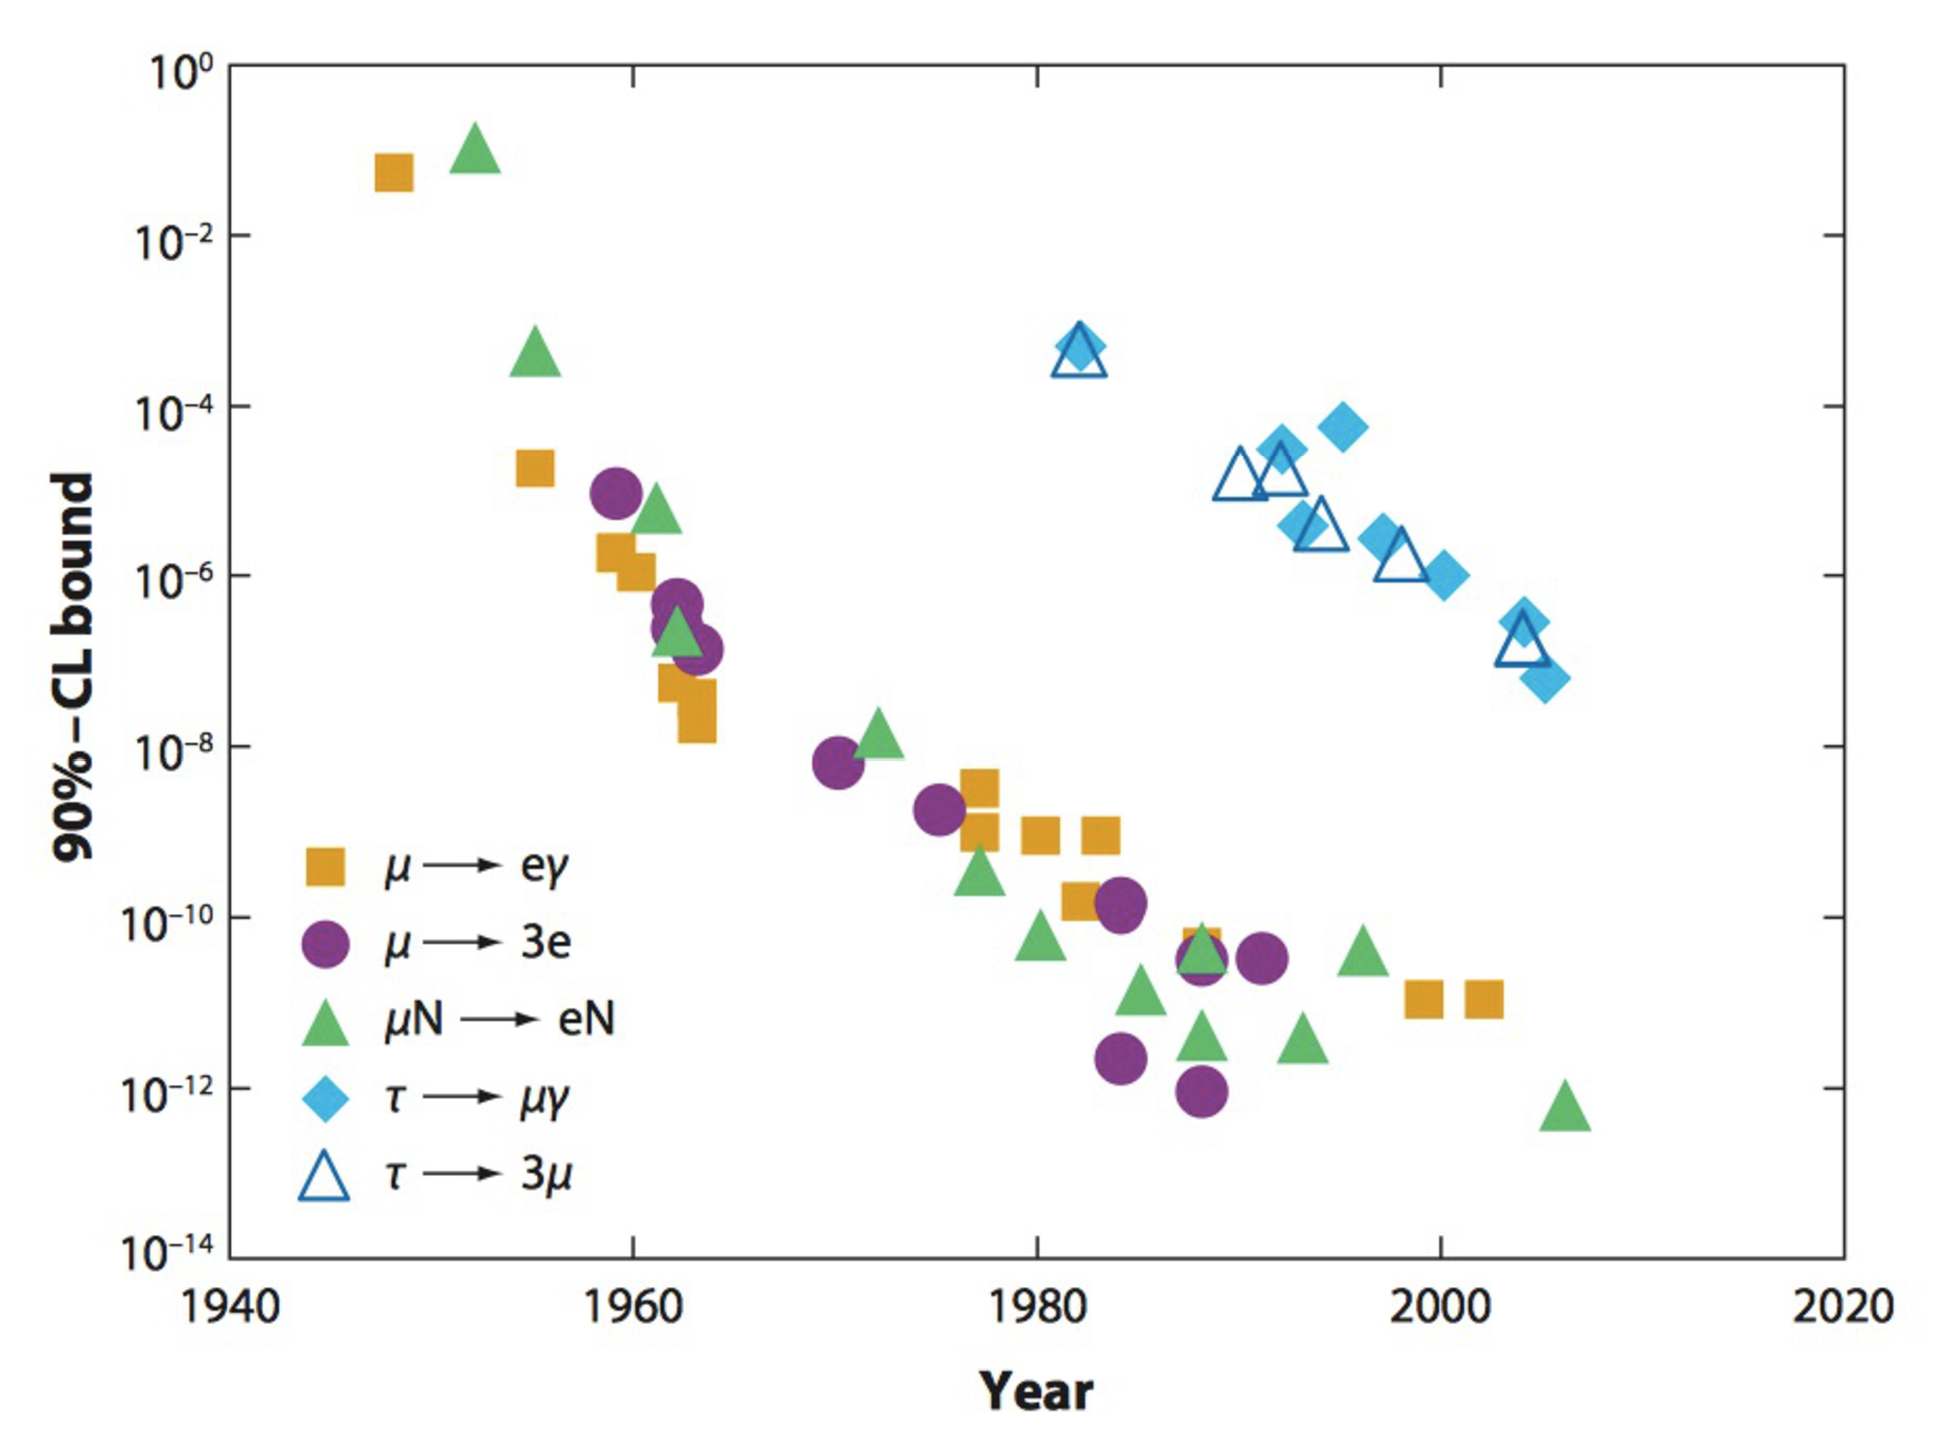
\includegraphics[width=0.7\textwidth]{Introduction/figs/LFV.pdf}
\caption{Summary of limits set in LFV searches as a function of time~\cite{Marciano:2008zz}.}
\label{fig:LFV_decay}
\end{figure}
 
